\chapter{Описание существующих решений}

\section{Python}

Python \cite{python} --- интерпретируемый язык программирования с сильной динамической типизацией. Официально язык был представлен в 1991 году. Существует множество реализаций интерпретатора языка Python \cite{juthon} \cite{ironpython} \cite{pypy}. Среди них канонической считается реализация CPython, разработанная на языке C и официально представленная в 1994 году. \cite{cpython}

Интерпретатор CPython использует механизм \textbf{GIL} (Global Interpreter Lock, глобальная блокировка интерпретатора), который обеспечивает однопоточное выполнение байт-кода Python. Этот механизм упрощает реализацию CPython, делая объектную модель (включая встроенные типы, такие как dict) неявно защищённой от конкурентного доступа и упрощая многопоточное выполнение программ. Однако некоторые модули расширения (как стандартные, так и сторонние) \cite{python_extensions} освобождают GIL при выполнении ресурсоёмких задач, таких как сжатие или хеширование. Кроме того, GIL всегда освобождается при выполнении ввода-вывода. \cite{gil}

\subsection{Выделение памяти}

Все объекты программы на языке Python размещаются в \textbf{приватной куче} (private heap), управление которой обеспечивается встроенным в интерпретатор диспетчером памяти. \cite{python_memory}

На самом низком уровне аллокатор необработанной памяти (raw memory allocator) взаимодействует с диспетчером памяти операционной системы и гарантирует, что в приватной куче есть достаточно места для хранения всех данных, используемых программой. Помимо аллокатора необработанной памяти используется несколько объектно-ориентированных аллокаторов, которые реализуют различные политики управления памятью, адаптированные к особенностям каждого типа данных. Диспетчер памяти Python делегирует часть работы объектно-ориентированным аллокаторам, гарантируя, что они работают в пределах приватной кучи. \cite{python_memory}

Для выделения памяти допускается использование как функций API Python/C, так и функций стандартной библиотеки языка C. В большинстве ситуаций рекомендуется выделять память в приватной куче, чтобы интерпретатор Python имел более точное представление об использовании памяти. \cite{python_memory}

Все функции распределения памяти в языке Python принадлежат одному из трёх \textbf{доменов} (PyMemAllocatorDomain). Эти домены представляют разные стратегии распределения и оптимизированы для разных целей. \cite{python_memory}

\begin{enumerate}[label*=\arabic*.]
	\item \textbf{Raw domain} предназначен для выделения памяти под буферы общего назначения в тех случаях, когда выделение должно передаваться системному аллокатору или когда аллокатор может работать без GIL. Память запрашивается непосредственно у операционной системы.
	\item \textbf{<<Mem>> domain} предназначен для выделения памяти для буферов Python и буферов общего назначения, где выделение должно выполняться с удержанием GIL. Память берётся из приватной кучи Python.
	\item \textbf{Object domain} предназначен для выделения памяти для объектов Python. Память берётся из приватной кучи Python.
\end{enumerate}

При освобождении памяти, ранее выделенной функциями, принадлежащими какому-либо домену, необходимо использовать соответствующие функции освобождения из того же домена. \cite{python_memory}



\subsection{Структура объекта}

Основной алгоритм сборки мусора, используемый CPython, --- подсчет ссылок. Для его реализации в структуре объекта Python предусмотрены поля, хранящие число ссылок и данные о типе объекта (\textbf{PyObject\_HEAD}), а также указатели на элементы двусвязного списка объектов, отслеживаемых сборщиком мусора (\textbf{PyGC\_Head}). Структура объекта Python представлена на рисунке \ref{fig:pyobject}.~\cite{python_gc}

\begin{figure}[H]
	\centering
	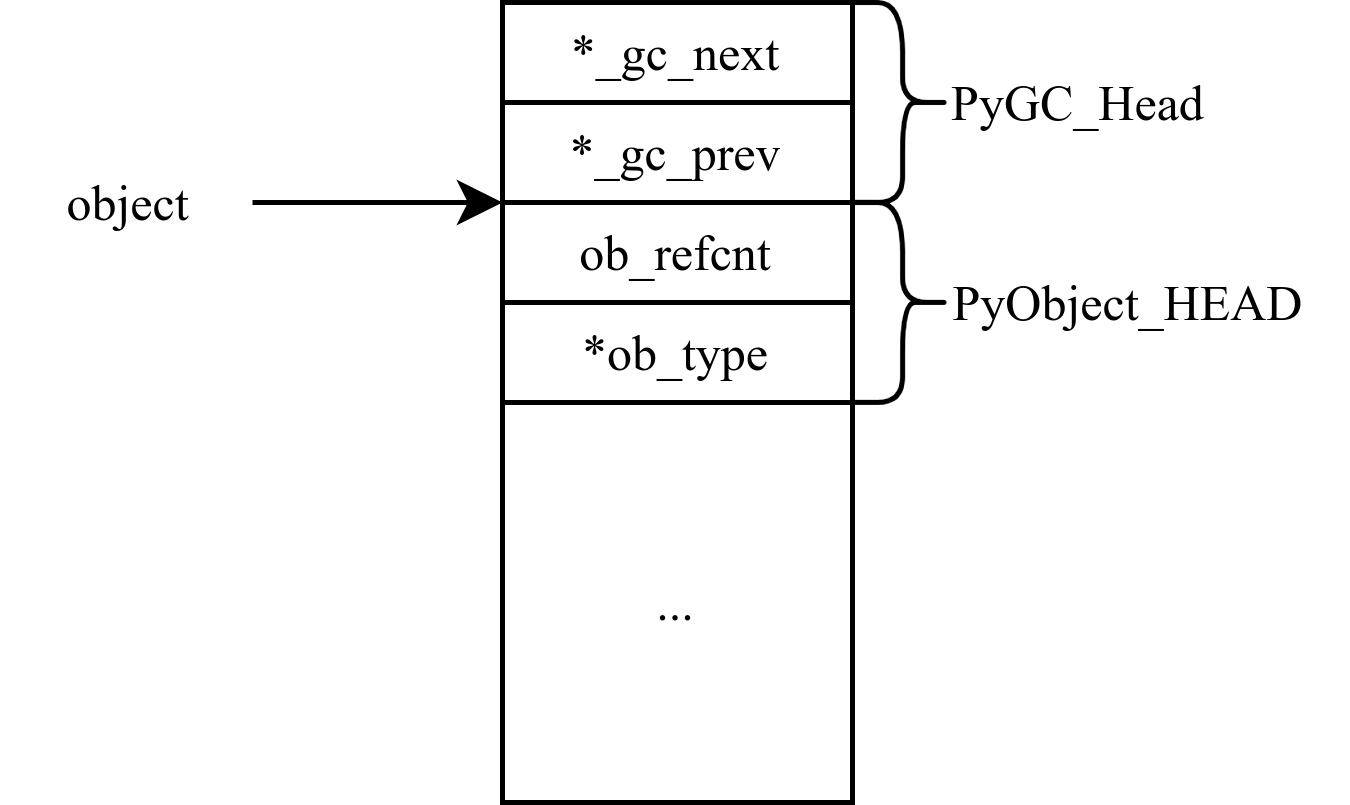
\includegraphics[scale=0.27]{assets/python-object.png}
	\caption{Структура объекта Python}
	\label{fig:pyobject}
\end{figure}

Когда необходима дополнительная информация, связанная со сборщиком мусора, к полям PyGC\_Head можно получить доступ с помощью адресной арифметики и приведения типа исходного объекта. \cite{python_gc}

Двусвязные списки используются по той причине, что они эффективно поддерживают операции, наиболее часто используемые при выполнении алгоритма сбора мусора, такие как перемещение объекта из одного раздела в другой, добавление нового объекта, полное удаление объекта, а также разбиение и объединение списков. \cite{python_gc}



\subsection{Сборка мусора}

Основная проблема подсчета ссылок заключается в том, что он не обрабатывает циклические ссылки. Для её решения используется отдельный сборщик мусора, который занимается только очисткой объектов-контейнеров, то есть объектов, которые могут содержать ссылки на другие объекты. \cite{python_gc}

На рисунках \ref{fig:python-gc} и \ref{fig:python-free} представлены схемы алгоритмов сборки мусора, которые обрабатывают циклические ссылки. \cite{python_gc}

\begin{figure}[H]
	\centering
	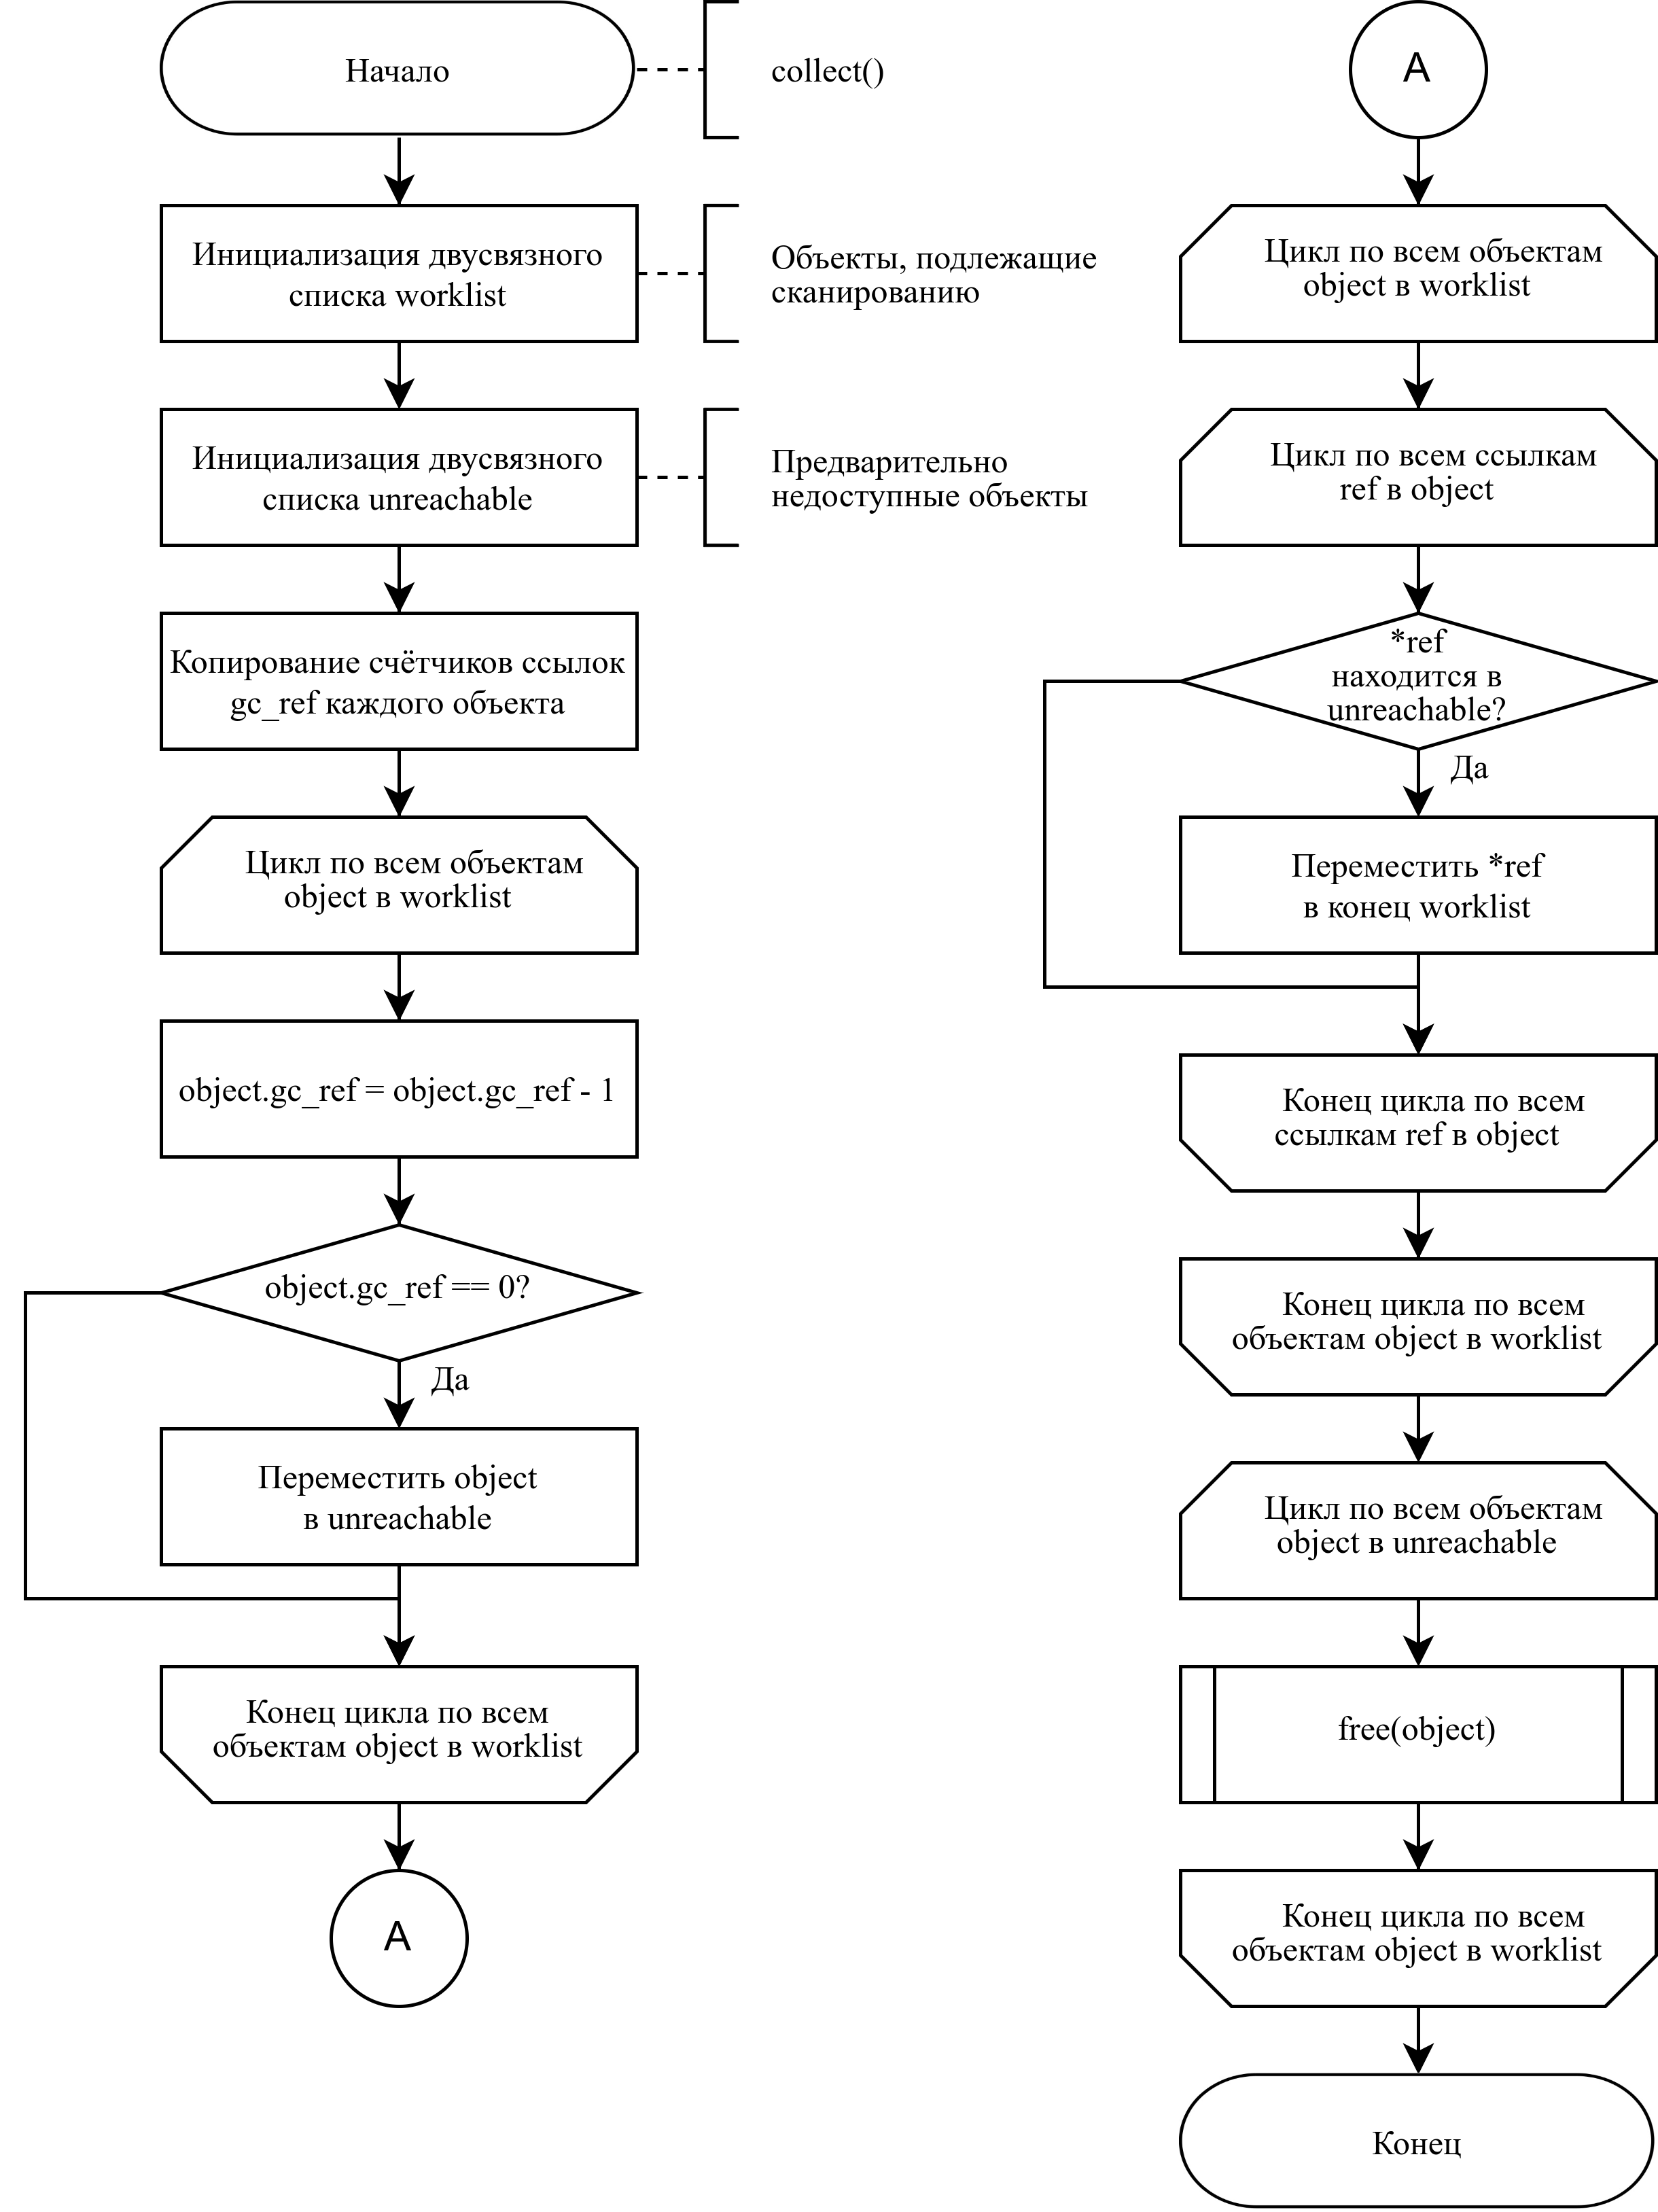
\includegraphics[scale=0.175]{assets/python-gc.png}
	\caption{Схема алгоритма сбора циклических ссылок}
	\label{fig:python-gc}
\end{figure}

\begin{figure}[H]
	\centering
	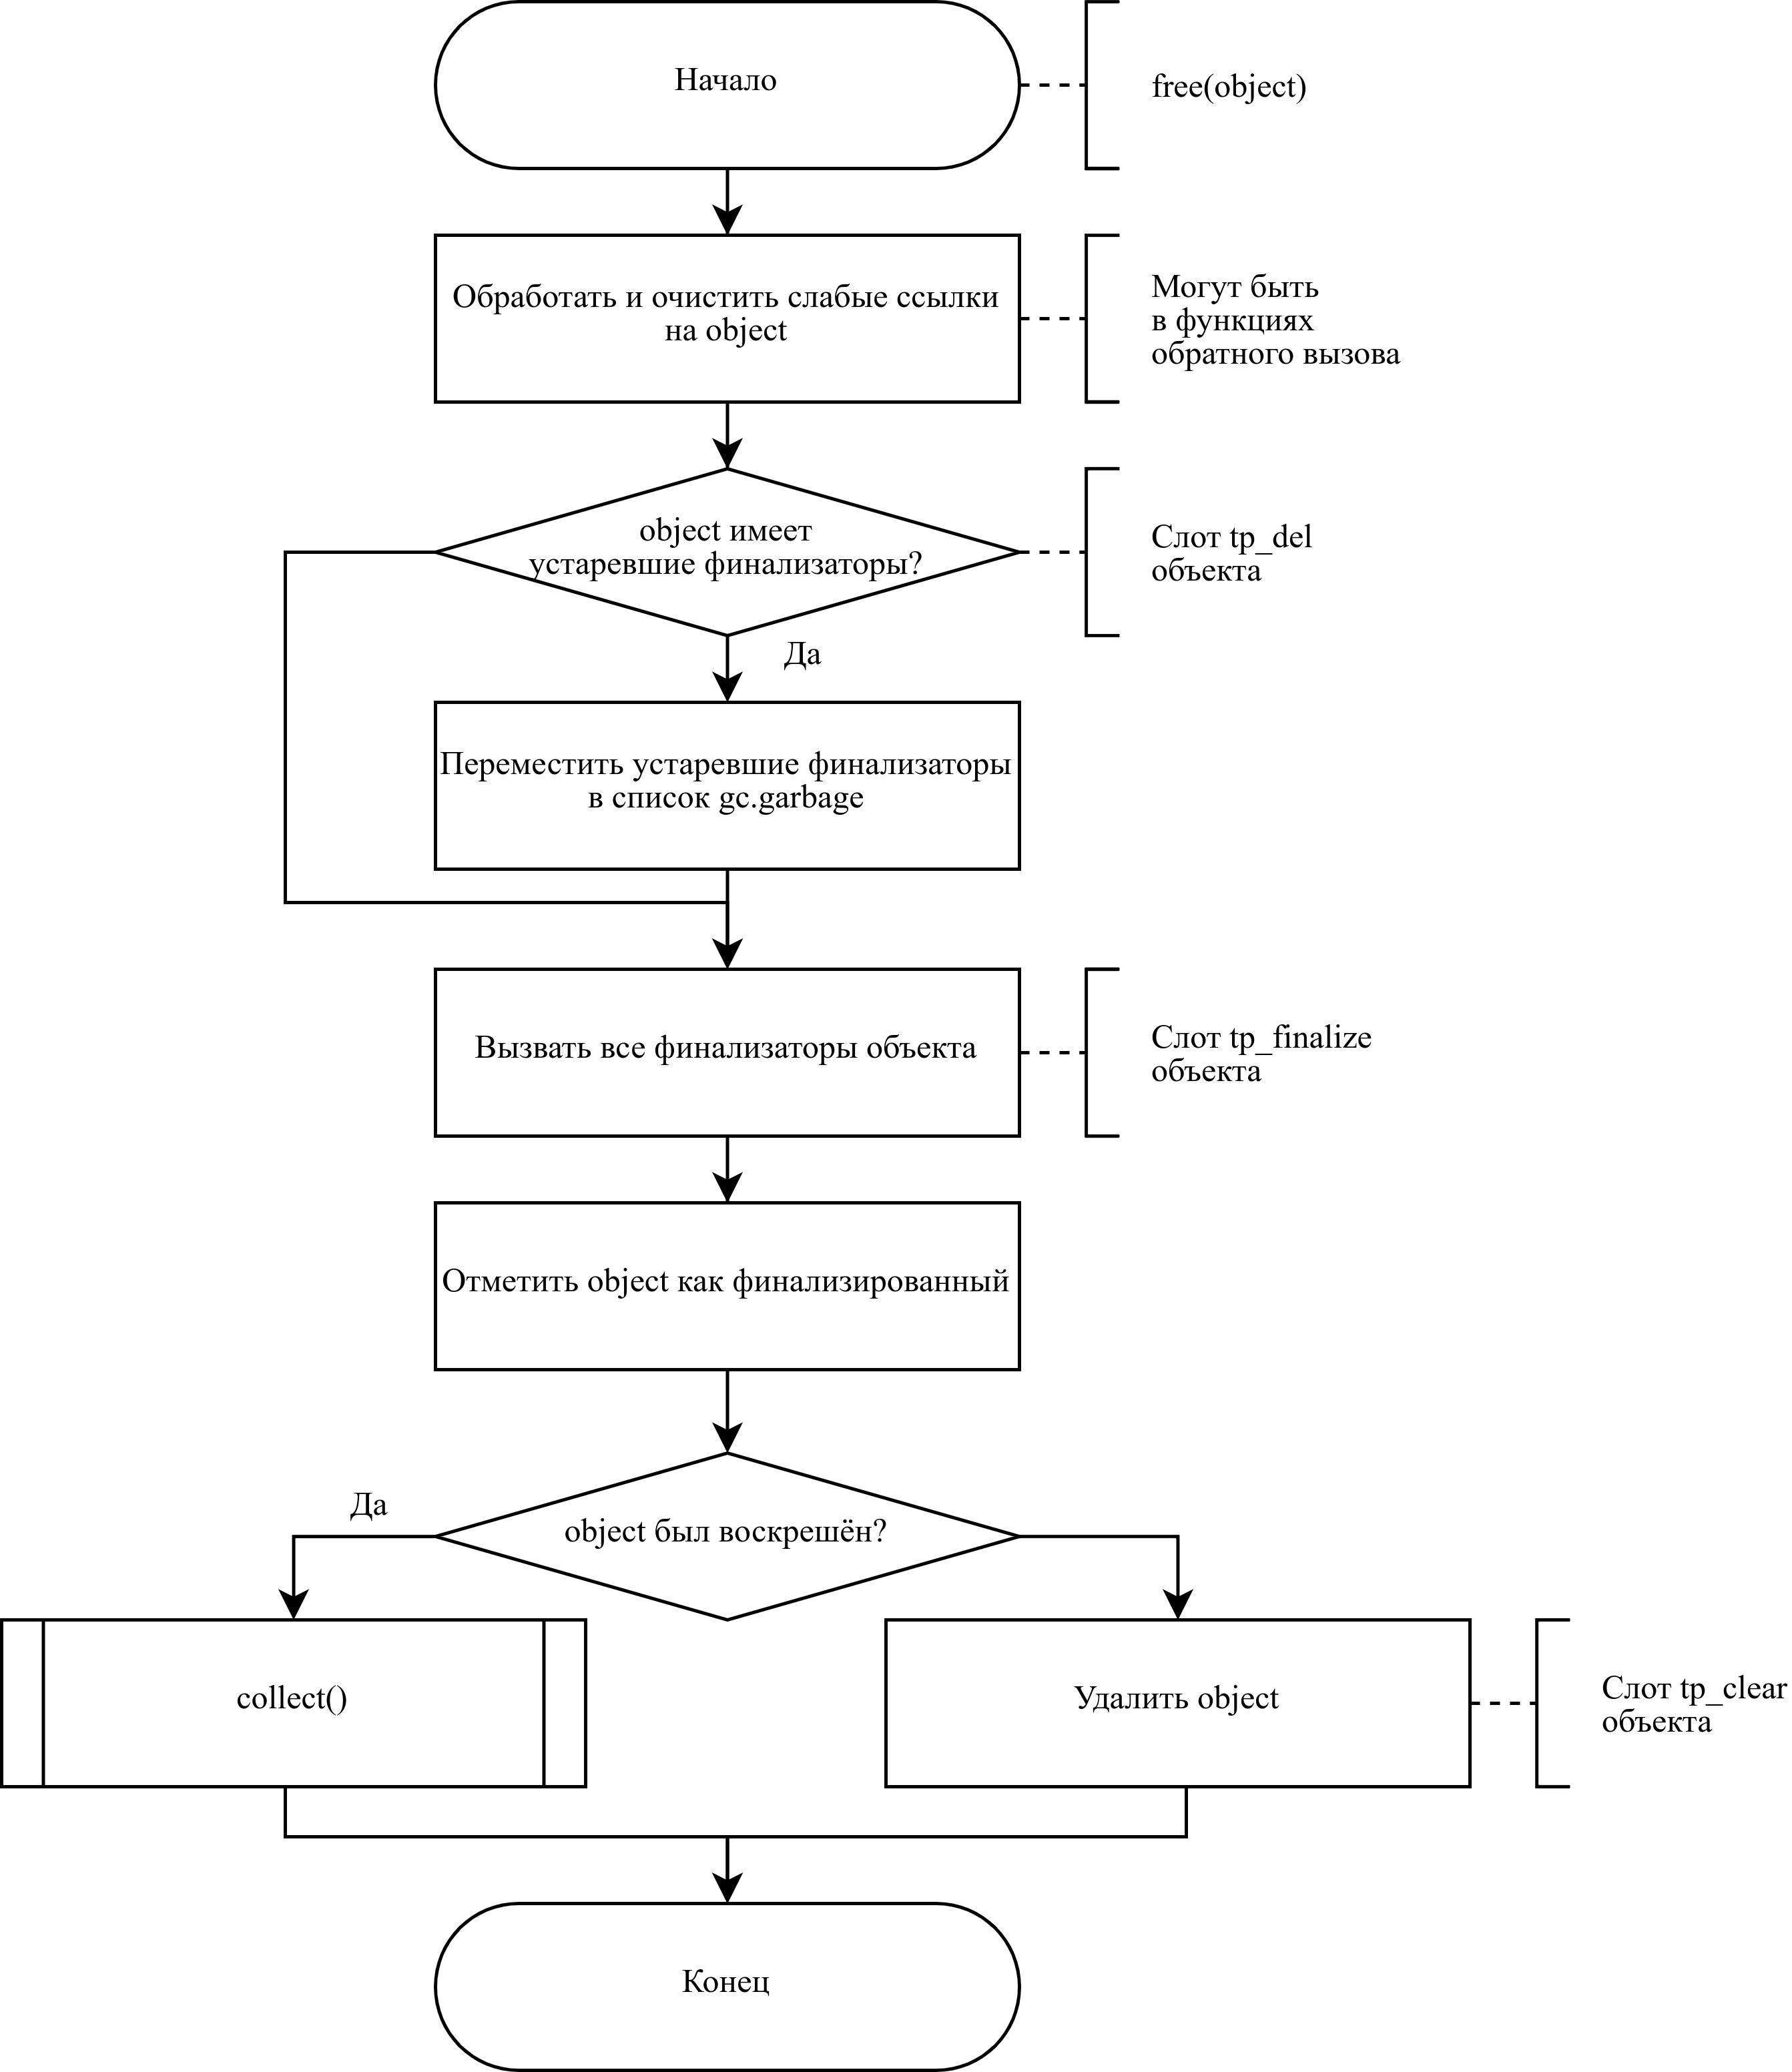
\includegraphics[scale=0.175]{assets/python-free.png}
	\caption{Схема алгоритма освобождения объекта}
	\label{fig:python-free}
\end{figure}

Стоит отметить, что такая сборка мусора выполняется конкурентно с основной программой в одном выделенном потоке сборщика, не распределяя работу по сборке на несколько потоков приложения. \cite{python_threaded_gc}



\subsection{Оптимизации}

Для снижения накладных расходов на сборку мусора в языке Python используются следующие оптимизации.

\begin{enumerate}[label*=\arabic*.]
	\item \textbf{Алгоритм поколений} (см. п. \ref{generational}). Для его реализации все объекты-контейнеры разделяются на три пространства (поколения). Каждый новый объект помещается в первое поколение. Алгоритм сбора мусора выполняется только над объектами определённого поколения, и если объект не уничтожается во время обработки своего поколения, он будет перемещён в следующее поколение, где его будут анализировать реже. Если тот же объект не уничтожается после ещё одного цикла сборки мусора, он будет перемещен в последнее поколение, где его будут анализировать реже всего. Чтобы определить момент запуска сбора мусора, сборщик отслеживает количество выделений и освобождений объектов с момента последнего сбора. Когда разность между ними превысит заданный порог (threshold), начнётся сбор. Первоначально исследуется только первое поколение. Если количество его сканирований после последнего анализа первого поколения превысило заданный порог, то также анализируется второе поколение. Последнее поколение сканируется только в том случае, если количество выделений объектов превышает количество освобождений на заданное значение (по умолчанию задано 25\%). \cite{python_gc}
	
	\item \textbf{Повторное использование полей ссылок}. В целях экономии памяти указатели из поля PyGC\_Head каждого объекта используются для нескольких целей. Эта оптимизация носит название <<толстые указатели>> (fat pointers) или <<теговые указатели>> (tag pointers). Так, внутрь указателей помещаются дополнительные данные с учётом следующего свойства адресации памяти: большинство архитектур выравнивают размеры типов данных по определённой величине, зачастую кратной машинному слову. Следовательно, несколько младших бит указателя всегда заполнены нулями и их можно использовать для хранения другой информации, чаще всего в виде битового поля. \cite{python_gc}
	
	\item \textbf{Задержка отслеживания контейнеров}. Определённые типы контейнеров не могут участвовать в цикле ссылок, поэтому сборщик мусора не отслеживает их. Существует два случая, когда отслеживание контейнера откладывается:
	\begin{itemize}[label*=---]
		\item когда контейнер создан;
		\item когда контейнер сканируется сборщиком мусора.
	\end{itemize}
	Как правило, экземпляры простых (атомарных) типов данных не отслеживаются, а экземпляры агрегированных типов (контейнеры, определяемые пользователем объекты и т.д.) отслеживаются. Тем не менее, могут быть предусмотрены некоторые оптимизации для конкретных типов, чтобы снизить влияние сборщика мусора на экземпляры простых типов. Так, кортежи (tuple) и словари (dict), содержащие только неизменяемые объекты (числа, строки, кортежи неизменяемых объектов и т.д.) не отслеживаются сборщиком мусора. \cite{python_gc}
\end{enumerate}

%Рассматриваем только реализацию Cython.
%
%https://docs.python.org/3/c-api/memory.html
%
%https://devguide.python.org/internals/garbage-collector/
%
%https://stackify.com/python-garbage-collection/
%
%https://realpython.com/python-memory-management/https://www.honeybadger.io/blog/memory-management-in-python/
%
%https://medium.com/analytics-vidhya/python-memory-management-8854f4952ba0
%
%https://scoutapm.com/blog/python-garbage-collection
%
%
%
%https://www.javatpoint.com/python-memory-management
%
%https://towardsdatascience.com/memory-management-and-garbage-collection-in-python-c1cb51d1612c
%
%https://rushter.com/blog/python-garbage-collector/
%
%https://scoutapm.com/blog/python-garbage-collection





\section{Java}

% https://www.oracle.com/webfolder/technetwork/tutorials/obe/java/gc01/index.html
Java \cite{java_gc_basics} --- компилируемый язык программирования с сильной статической типизацией. Официально был представлен в 1995 году компанией Sun Microsystems. 

% https://www.oracle.com/webfolder/technetwork/tutorials/obe/java/gc01/index.html
Среда выполнения языка Java (Java Runtime Environment, JRE) состоит из \textbf{виртуальной машины Java} (Java Virtual Machine, JVM), основных классов и вспомогательных библиотек платформы Java. Рассматриваемый язык является кроссплатформенным: приложения, разработанные на Java, компилируются в \textbf{байт-код}, который сохраняется в файлах классов и запускается в JVM. Поэтому программы на языке Java можно запустить на всех аппаратных платформах и операционных системах, для которых реализована JVM. \cite{java_gc_basics}



\subsection{Виртуальная машина Java}

% https://docs.oracle.com/javase/specs/jvms/se21/html/jvms-1.html
Виртуальная машина Java (JVM) является основой платформы Java. Это компонент технологии, отвечающий за её независимость от аппаратного обеспечения и операционной системы, минимальный размер скомпилированного исполняемого кода и безопасность. \cite{java_21_spec}

% https://docs.oracle.com/javase/specs/jvms/se21/html/jvms-1.html
Виртуальная машина Java \cite{java_21_spec} --- это абстрактная вычислительная машина. Как и реальная вычислительная машина, она имеет набор команд и управляет различными областями памяти во время выполнения.

% https://docs.oracle.com/javase/specs/jvms/se21/html/jvms-1.html
Современные реализации Oracle JVM эмулируют работу виртуальной машины Java на мобильных, настольных и серверных устройствах, но виртуальная машина Java не предполагает какой-либо конкретной технологии реализации, аппаратного обеспечения или операционной системы компьютера. JVM по своей сути не является интерпретатором, но может быть реализована путем компиляции её набора команд в набор команд процессора. \cite{java_21_spec}

% https://docs.oracle.com/javase/specs/jvms/se21/html/jvms-1.html
JVM ничего не знает о языке программирования Java и работает только с файлами классов в двоичном формате. Файл класса содержит инструкции JVM (байт-код) и вспомогательную информацию. \cite{java_21_spec} В целях безопасности виртуальная машина Java накладывает строгие синтаксические и структурные ограничения на код в файле класса. Однако любой язык, функциональность которого может быть выражена в виде допустимого файла класса, может размещаться на виртуальной машине Java. По этой причине разработчики могут использовать JVM в качестве машинно-независимой платформы для запуска приложений, разработанных на языках программирования, совместимых с JVM. \cite{java_jvm_languages}
% https://www.oracle.com/technical-resources/articles/java/architect-languages.html

% https://openjdk.org/groups/hotspot/
Существует множество реализаций JVM. \cite{java_j9} \cite{java_codename_one} \cite{java_graalvm}
% https://eclipse.dev/openj9/
% https://www.codenameone.com/
% https://www.graalvm.org/
Среди них наиболее распространённой является HotSpot JVM, представленная в 1999 году компанией Sun Microsystems. \cite{java_hotspot} % https://openjdk.org/groups/hotspot/



\subsection{Управление памятью}

% https://openjdk.org/groups/hotspot/docs/StorageManagement.html
Частью JVM является \textbf{менеджер хранилища} (storage manager), который отвечает за управление жизненным циклом объектов Java: выделение новых объектов, сбор недоступных объектов и отправка уведомлений о недоступности по запросу. Виртуальная машина HotSpot предоставляет несколько менеджеров хранилища для удовлетворения потребностей различных типов приложений, обеспечивая короткие паузы в работе приложения и высокую пропускную способность. \cite{java_storage_management}

% https://openjdk.org/groups/hotspot/docs/StorageManagement.html
Основной структурой данных HotSpot JVM является \textbf{иерархия классов} (klass hierarchy), которая описывает объекты в хранилище виртуальной машины и обеспечивает операции над этими объектами. Иерархия классов поддерживает объектно-ориентированную парадигму языка Java, предоставляя механизм для методов объектов (в том числе виртуальных). \cite{java_storage_management}

% https://openjdk.org/groups/hotspot/docs/StorageManagement.html
Из соображений масштабируемости, каждый поток JVM имеет собственную область выделения памяти --- \textbf{буфер выделения потока} (Thread-Local Allocation Buffers, TLAB). Каждый поток может выделять ресурсы из своей TLAB без координации с другими потоками, за исключением случаев, когда ему требуется новая TLAB. \cite{java_storage_management}

% https://openjdk.org/groups/hotspot/docs/StorageManagement.html
Было замечено, что большинство программ на языке Java следует гипотезе поколений (см. п. \ref{generational}). Чтобы учесть это свойство программ при распределении памяти, объекты Java разделяются на три поколения: молодое (young), старое (old) и постоянное (permanent). Управление поколениями может осуществляться по различным алгоритмам. Предполагается, что в молодом поколении будет больше объектов, чем в старом, а также будет выше плотность недоступных объектов. \cite{java_storage_management}

% https://openjdk.org/groups/hotspot/docs/StorageManagement.html
\textbf{Молодое поколение} должно поддерживать быстрое распределение, при это ожидается, что большинство этих объектов относительно быстро станет недоступным. При сборе мусора в молодом поколении выявляются все достижимые объекты и копируются в старое поколение. Далее объекты, оставшиеся в молодом поколении, освобождаются. \cite{java_storage_management}

% https://openjdk.org/groups/hotspot/docs/StorageManagement.html
Идентификация достижимости в молодом поколении осуществляется без просмотра всего графа объектов. Решение данной задачи основывается на гипотезе поколений, согласно которой имеется мало ссылок от старых объектов к молодым. JVM сохраняет <<запоминаемый набор>> (remembered set) ссылок от старого поколения к молодому и использует его для обхода объектов молодого поколения. \cite{java_storage_management}

% https://openjdk.org/groups/hotspot/docs/StorageManagement.html
% https://www.oracle.com/technetwork/java/javase/memorymanagement-whitepaper-150215.pdf
Объекты в \textbf{старом поколении} могут анализироваться сборщиком мусора реже, чем объекты в молодом поколении. Также сборщик мусора в зависимости от выбранной стратегии выполнять копирование и уплотнение объектов. Данная операция повышает накладные расходы на сборку мусора, поскольку необходимо перемещать объекты и обновлять все ссылки на объект, чтобы они указывали на новое местоположение объекта. С другой стороны, копирование объектов означает, что можно аккумулировать освобождённое пространство в один большой регион, из которого выделение происходит быстрее (что ускоряет очистку молодого поколения), а также появляется возможность вернуть избыточную память операционной системе. \cite{java_storage_management} \cite{java_memory}

% https://openjdk.org/groups/hotspot/docs/StorageManagement.html
Помимо объектов, созданных программой на языке Java, существуют объекты, созданные и используемые JVM. Чтобы не путать их с объектами выполняемой программы, такие объекты выделяют в \textbf{постоянное поколение}. Данное название носит исторический характер и на самом деле объекты в нём не существуют на протяжении всего времени выполнения программы. Например, информация о загруженных классах хранится в постоянном поколении и уничтожается, когда эти классы больше не доступны из приложения. \cite{java_storage_management}

% https://www.oracle.com/webfolder/technetwork/tutorials/mooc/JVM_Troubleshooting/week1/lesson1.pdf
Начиная с Java 8 постоянное поколение было заменено \textbf{метапространством} (MetaSpace), предназначенным для хранения классов и метаданных JVM.~\cite{java_presentation}



\subsection{Сборка мусора}

% https://docs.oracle.com/en/java/javase/21/gctuning/available-collectors.html
HotSpot JVM предоставляет несколько сборщиков мусора, оптимизированных для различных типов приложений. Далее будут рассмотрены сборщики мусора, доступные в Java 21. \cite{java_21_available_collectors}
% https://docs.oracle.com/en/java/javase/21/



\subsubsection{Serial Collector}
% https://docs.oracle.com/en/java/javase/21/gctuning/available-collectors.html
Serial Collector работает по алгоритму mark-compact (см. п. \ref{mark-compact}) и использует один поток для выполнения основной и второстепенной работы по сбору мусора, что может повысить его эффективность за счёт отсутствия накладных расходов на взаимодействие параллельных потоков. \cite{java_21_available_collectors}

% https://docs.oracle.com/en/java/javase/21/gctuning/available-collectors.html
Он лучше всего подходит для однопроцессорных вычислительных машин, поскольку не может использовать преимущества многопроцессорного оборудования, хотя может быть полезен на многопроцессорных системах для приложений с небольшими наборами данных (приблизительно до 100 МБ). \cite{java_21_available_collectors}

% https://www.oracle.com/webfolder/technetwork/tutorials/obe/java/gc01/index.html
Также Serial Collector используется в том случае, когда на одной машине работает большое количество JVM, которое может превышать количество доступных процессоров. В таких средах рекомендуется использовать только один процессор для сборки мусора, чтобы минимизировать влияние виртуальных машин друг на друга, жертвуя увеличением времени сборки мусора. \cite{java_gc_basics}

% https://www.oracle.com/webfolder/technetwork/tutorials/obe/java/gc01/index.html
% Наконец, с распространением встроенного оборудования с минимальным объемом памяти и несколькими ядрами, Serial GC может вернуться.


\subsubsection{Parallel Collector}

% https://docs.oracle.com/en/java/javase/21/gctuning/available-collectors.html
Parallel Collector отличается от Serial Collector использованием нескольких потоков для сборки мусора, количество которых может регулироваться с помощью аргументов командной строки. \cite{java_21_available_collectors} По умолчанию количество используемых потоков равно количеству доступных процессоров. \cite{java_gc_basics}
% https://www.oracle.com/webfolder/technetwork/tutorials/obe/java/gc01/index.html
Во время работы Parallel Collector все потоки основной программы приостанавливаются (<<stop the world>>, см. п. \ref{mark-sweep}). \cite{java_jrockit_memory}
% https://docs.oracle.com/cd/E15289_01/JRSDK/garbage_collect.htm

% https://www.oracle.com/webfolder/technetwork/tutorials/obe/java/gc01/index.html
На однопроцессорной машине используется сборщик мусора по умолчанию, даже если был выбран Parallel Collector. На машине с двумя процессорами он сопоставим по производительности со сборщиком мусора по умолчанию. На вычислительных машинах с большим количеством процессоров можно ожидать сокращения времени паузы на сборку мусора. \cite{java_gc_basics}

% https://www.oracle.com/webfolder/technetwork/tutorials/obe/java/gc01/index.html
Parallel Collector также называют Throughput Collector, так как он может использовать несколько процессоров для ускорения сборки мусора и повышения пропускной способности при работе с памятью, что повышает производительность приложений. \cite{java_gc_basics} Рассматриваемый сборщик мусора следует использовать на многопроцессорном оборудовании, когда необходимо выполнить относительно большой объём работы и допустимы длинные паузы. Например, при пакетной обработке (batch processing), такой как печать документов или выполнение большого количества запросов к базе данных. \cite{java_21_available_collectors}
% https://docs.oracle.com/en/java/javase/21/gctuning/available-collectors.html


\subsubsection{Garbage-First Collector}

% https://docs.oracle.com/en/java/javase/21/gctuning/available-collectors.html
% G1 — это в основном параллельный сборщик. В большинстве случаев параллельные сборщики выполняют некоторую дорогостоящую работу одновременно с приложением. Этот сборщик предназначен для масштабирования от небольших машин до больших многопроцессорных машин с большим объемом памяти. Это обеспечивает возможность достижения цели по времени паузы с высокой вероятностью при достижении высокой пропускной способности.

% https://www.oracle.com/java/technologies/javase/hotspot-garbage-collection.html
Garbage-First Collector (также G1) --- это сборщик мусора, работающий по алгоритму mark-sweep (см. п. \ref{mark-sweep}), предназначенный для многопроцессорных машин с большим объемом памяти. Он с высокой вероятностью соответствует целевому времени паузы для сборки мусора, обеспечивая при этом относительно высокую пропускную способность. Операции над всей кучей, такие как глобальная разметка объектов, выполняются конкурентно с потоками приложения. Это предотвращает паузы в работе приложений, пропорциональные размеру кучи и используемых данных. \cite{java_g1}

Начиная с версии Java 9, Garbage-First Collector выбирается по умолчанию в большинстве конфигураций оборудования и операционной системы или может быть явно включён с помощью параметров командной строки. \cite{java_g1}

% https://www.oracle.com/java/technologies/javase/hotspot-garbage-collection.html
Garbage-First Collector достигает высокой производительности при снижении длительности пауз за счет применения следующих методов. \cite{java_g1}

\begin{enumerate}[label*=\arabic*.]
	\item В отличие от Parallel Collector работа потоков приостанавливается только на некоторые этапы сборки мусора: в начале при разметке объектов из корневого набора (см. п. \ref{roots}) и в конце при обнаружении изменений, произошедших за время сборки мусора. \cite{java_jrockit_memory} % https://docs.oracle.com/cd/E15289_01/JRSDK/garbage_collect.htm
	\item Куча разделяется на набор непрерывных областей одинакового размера, называемых регионами. Garbage-First Collector выполняет конкурентную фазу глобальной разметки для обнаружения используемых объектов в куче, после чего определяет, какие регионы <<почти пусты>> (mostly empty). Именно в этих регионах в первую очередь будет выполняться сбор мусора и уплотнение неиспользуемых объектов, чтобы как можно раньше дать аллокатору непрерывные свободные области памяти наибольшего размера. Garbage-First Collector концентрирует свою деятельность по сбору и уплотнению на тех областях кучи, которые, предположительно, будут заполнены неиспользуемыми объектами. 
	\item Используется \textbf{модель прогнозирования паузы} (pause prediction model) для достижения заданного пользователем целевого времени паузы на сборку мусора и на его основе выбирает количество регионов для обработки.
	\item В отличие от Parallel Collector используемые объекты выбираются для копирования и уплотнения не из всей кучи, а только из некоторых её областей. Эта операция выполняется параллельно на нескольких процессорах, чтобы уменьшить время паузы на сборку мусора и увеличить пропускную способность. Таким образом, при каждой сборке мусора G1 непрерывно работает над уменьшением фрагментации кучи, работая в течение заданного пользователем времени паузы.
\end{enumerate}

% https://www.oracle.com/java/technologies/javase/hotspot-garbage-collection.html
Важно отметить, что Garbage-First Collector не является сборщиком мусора в режиме реального времени. Вероятность соответствия заданному целевому времени паузы высока, но не равна единице. На основе данных о предыдущих циклах сборки мусора Garbage-First Collector оценивает, сколько регионов можно освободить в течение заданного пользователем целевого времени с помощью модели определения накладных расходов на обработку каждого региона.~\cite{java_g1}


\subsubsection{Z Garbage Collector}

% https://wiki.openjdk.org/display/zgc/Main
Z Garbage Collector (также ZGC) --- это сборщик мусора, работающий по алгоритму mark-compact (см. п. \ref{mark-compact}) и нацеленный на минимизацию пауз. ZGC работает конкурентно с основной программой, не останавливая выполнение потоков приложения более чем на миллисекунду, при этом жертвуя пропускной способностью. Он предназначен для приложений, которым требуется низкая задержка на сборку мусора. Время пауз не зависит от размера используемых данных в куче. ZGC оптимизирован для работы с кучей размером от нескольких сотен мегабайт до 16 Тб. \cite{java_zgc}

% https://wiki.openjdk.org/display/zgc/Main
Первоначально ZGC был представлен как экспериментальная опция в Java 11 и стал полноценной частью JVM в Java 15. \cite{java_zgc} Начиная с Java 21 поддерживает опцию использования алгоритма поколений. \cite{java_21_available_collectors}
% https://docs.oracle.com/en/java/javase/21/gctuning/available-collectors.html

% https://wiki.openjdk.org/display/zgc/Main
Ниже представлены основные характеристики Z Garbage Collector. \cite{java_zgc}

\begin{enumerate}[label*=\arabic*.]
	\item Сборка мусора выполняется конкурентно с основной программой.
	
	\item Куча разделяется на регионы для дальнейшего уплотнения, как при работе Garbage-First Collector.
	
	\item Используются \textbf{цветные указатели} (colored pointers): ZGC поддерживает только 64-битные указатели и хранит в них не только адрес объекта в памяти, но и дополнительные метаданные, определяющие текущий статус указателя:
	\begin{itemize}[label*=---]
		\item Marked0 и Marked1 --- фаза сборки мусора;
		\item Remapped --- адрес в указателе является окончательным и не должен модифицироваться в рамках текущего цикла сборки;
		\item Finalizable --- объект достижим только из финализатора.
	\end{itemize}

	\item Во время конкуррентных фаз сборки мусора используются \textbf{барьеры} (barriers) --- функции, которые принимают указатель на объект в памяти, анализирует его статус, в зависимости от него выполняют какие-либо действия с этим указателем или даже с объектом, на который он ссылается, после чего возвращают актуальное значение указателя, которое можно использовать для доступа к объекту.
\end{enumerate}

Важной особенностью барьера является то, что он выполняется в том числе в потоках основной программы. То есть сборкой мусора занимаются не только выделенные потоки сборщика, но и само приложение.


\subsubsection{Выбор сборщика мусора}

% https://docs.oracle.com/en/java/javase/11/gctuning/available-collectors.html
Сборщик мусора для JVM следует выбирать для каждого приложения отдельно, поскольку производительность сбора мусора зависит от размера кучи, объёма используемых данных, а также от количества и характеристик доступных процессоров. Однако можно сформировать некоторые рекомендации, которые послужат отправной точкой для выбора сборщика. \cite{java_11_available_collectors}

\begin{enumerate}[label*=\arabic*.]
	\item Если приложение не имеет довольно строгих требований к времени паузы, сначала запустите приложение и позвольте виртуальной машине выбрать сборщик.
	\item Если приложение работает с относительно небольшим набором данных (приблизительно до 100 Мб), следует выбрать Serial Collector.
	\item Если приложение будет запускаться на одном процессоре и нет требований к времени паузы, следует выбрать Serial Collector.
	\item Если пиковая производительность приложения является главным приоритетом и нет требований к времени паузы, то есть паузы длительностью более одной секунды приемлемы, тогда следует выбрать сборщик по умолчанию или Parallel Collector.
	\item Если время ответа на запрос выделения памяти более важно, чем общая пропускная способность, а паузы для сбора мусора должны быть короче, следует выбрать Garbage-First Collector.
	\item Если время ответа имеет высокий приоритет, следует выбрать Z Garbage Collector.
\end{enumerate}



%https://www.amazon.com/dp/0137142528
%
%https://www.amazon.com/dp/1420082795
%
%
%
%https://en.wikipedia.org/wiki/Garbage-first_collector
%
%
%
%https://docs.oracle.com/cd/E13150_01/jrockit_jvm/jrockit/geninfo/diagnos/garbage_collect.html
%
%https://www.oracle.com/technetwork/java/javase/tech/memorymanagement-whitepaper-1-150020.pdf
%
%https://www.oracle.com/webfolder/technetwork/tutorials/obe/java/gc01/index.html
%
%https://docs.oracle.com/en/java/javase/11/gctuning/garbage-collector-implementation.html
%
%https://docs.oracle.com/javase/8/docs/technotes/guides/vm/gctuning/toc.html
%
%https://docs.oracle.com/javase/specs/jls/se8/html/jls-17.html
%
%https://www.oracle.com/technetwork/tutorials/tutorials-1876574.html
%
%
%
%https://openjdk.org/jeps/0
%
%
%
%https://cyberleninka.ru/article/n/java-garbage-collectors/viewer
%
%
%
%https://www.javatpoint.com/memory-management-in-java
%
%https://opensource.com/article/22/7/garbage-collection-java
%
%https://www.baeldung.com/java-choosing-gc-algorithm
%
%https://www.baeldung.com/jvm-garbage-collectors
%
%https://developers.redhat.com/articles/2021/11/02/how-choose-best-java-garbage-collector
%
%https://developers.redhat.com/articles/2021/08/20/stages-and-levels-java-garbage-collection
%
%https://howtodoinjava.com/java/garbage-collection/revisiting-memory-management-and-garbage-collection-mechanisms-in-java/
%
%https://howtodoinjava.com/java/garbage-collection/all-garbage-collection-algorithms/
%
%
%
%https://assets.ctfassets.net/oxjq45e8ilak/2K7aShH1CgWcUMc4Yqyg0g/b2606c497f7ac0a6bdc36c7c9ba910a1/be-prepared-to-g1-gc-or-evolution-of-the-g1-gc.pdf
%
%
%
%https://habr.com/ru/articles/269621/
% 
%https://habr.com/ru/articles/680038/
%
%https://java-ru-blog.blogspot.com/2020/01/garbage-first-g1-java-vm.html
%
%https://java-online.ru/garbage-collection.xhtml





\section{JavaScript}

JavaScript \cite{js} --- интерпретируемый язык программирования со слабой динамической типизацией, представленный в 1995 году. Стандартом языка является ECMAScript. \cite{ecmascript}

Наиболее широкое применение JavaScript получил в качестве языка сценариев веб-страниц, но также используется и в других программных продуктах, таких как node.js \cite{node_js} и Apache CouchDB \cite{couchdb}.



\subsection{Цикл событий}

\textbf{Модель времени выполнения} (runtime model) в JavaScript основана на \textbf{цикле событий} (event loop), который отвечает за сбор и обработку событий, а также за выполнение подзадач из очереди (queued sub-tasks). Далее будет описана теоретическая модель цикла событий, которую реализуют современные движки JavaScript, при этом, как правило, оптимизируя её семантику. \cite{js_event_loop}

Вызов любой функции создаёт контекст выполнения (Execution Context). При вызове вложенной функции создаётся новый контекст, а старый сохраняется в специальной структуре данных --- стеке вызовов (Call Stack). Объекты размещаются в куче. Также среда выполнения JavaScript содержит очередь задач, подлежащих обработке. Каждая задача ассоциируется с некоторым обработчиком (функцией). Обработка задачи заканчивается, когда стек снова становится пустым. Следующая задача извлекается из очереди и начинается её обработка. Каждая задача выполняется полностью, прежде чем начнёт выполняться следующая. Благодаря этому можно гарантировать, что выполнение функции не может быть приостановлено и будет завершено до начала выполнения другого кода (который может изменить данные, с которыми работает текущая функция). У данного подхода есть недостатки: если задача занимает слишком много времени, то веб-приложение не может обрабатывать действия пользователя в это время. В таких случаях современные браузеры выводят сообщение <<скрипт выполняется слишком долго>> (<<a script is taking too long to run>>) и предлагает остановить его. Хорошей практикой считается создание задач, которые исполняются относительно быстро и, если возможно, разбиение одной задачи на несколько подзадач. \cite{js_event_loop}

В браузерах события добавляются в очередь в любое время, если событие произошло, а так же если у него есть обработчик. В том случае, если у события нет обработчика, оно теряется. \cite{js_event_loop}

Для запуска скриптов в фоновом потоке предназначен \textbf{Web Worker} \cite{js_web_workers}. Поток Web Worker может выполнять задачи без вмешательства в пользовательский интерфейс, а также осуществлять ввод-вывод. Web Worker имеет свой собственный стек, кучу и очередь событий. Потоки событий можно связать друг с другом через отправку сообщений, добавляя их в соответствующие очереди.~\cite{js_event_loop}

Поток выполнения цикла событий в JavaScript никогда не блокируется. Выполнение ввода-вывода обычно осуществляется асинхронно с помощью событий и функций обратного вызова, поэтому, например, когда приложение ожидает ответа на запрос по сети, оно может обрабатывать другие задачи, например пользовательский ввод. \cite{js_event_loop}



\subsection{Сборка мусора}

Изначально интерпретаторы JavaScript использовали сборку мусора на основе подсчёта ссылок, не обрабатывая циклические ссылки, что могло приводить к систематическим утечкам памяти. По этой причине, начиная с 2012 года, все современные веб-браузеры оснащаются сборщиками мусора, работающими исключительно по алгоритму mark-sweep (см. п. \ref{mark-sweep}). Все усовершенствования алгоритма сборки мусора в интерпретаторах JavaScript (инкрементальная, конкурентная и параллельная сборка мусора, а также применение алгоритма поколений) за последние несколько лет представляют собой усовершенствования данного алгоритма, не являясь новыми алгоритмами сборки мусора, поскольку дальнейшее сужение понятия <<объект более не используется>> не представляется возможным. \cite{js_memory}



\subsection{Вспомогательные структуры данных}

Хотя JavaScript не предоставляет напрямую API сборщика мусора, язык предлагает несколько структур данных, которые косвенно наблюдают за сборкой мусора и могут использоваться для управления использованием памяти.~\cite{js_memory}

\textbf{WeakMap} и \textbf{WeakSet} (<<слабые>> аналоги Map и Set) позволяют поддерживать коллекцию пар ключ-значение и коллекцию уникальных значений соответственно. Эти структуры данных получили своё название от концепции слабо удерживаемых значений. Объект X слабо удерживается объектом Y, если имеется возможность получить доступ к значению X через Y, при этом алгоритм сборки мусора не будет считать X достижимым, если он не удерживается никакими другими объектами. Большинство структур данных, за исключением WeakMap, WeakSet и WeakRef, строго привязаны к вложенным объектам, поэтому их можно получить в любой момент. Ключи WeakMap и WeakSet могут быть очищены сборщиком мусора (для объектов WeakMap значения также будут подлежать сбору мусора), если ничто другое в программе не ссылается на них. Это обеспечивается следующими характеристиками. \cite{js_memory}

\begin{itemize}[label*=---]
	\item WeakMap и WeakSet могут хранить только объекты или символы, так как сборке мусора подлежат только они.
	\item WeakMap и WeakSet не являются итерируемыми (iterable).
\end{itemize}

Стоит отметить, что в программах на JavaScript допускается случай, когда значение ссылается на ключ. Так будет создана циклическая ссылка, которая сделает невозможным сбор мусора как для ключа, так и для значения, даже если ничто другое не ссылается на ключ. Чтобы исправить это, записи в WeakMap и WeakSet являются не реальными ссылками, а \textbf{эфемеронами} (ephemerons), что является усовершенствованием алгоритма mark-sweep. Эфемероны \cite{js_ephemerons}--- это уточнение слабых пар, в которых ни ключ, ни значение не могут быть классифицированы как слабые или сильные. Связность ключа определяет связность значения, но связность значения не влияет на связность ключа. Если сборка мусора предлагает поддержку эфемеронов, то она проходит в три этапа вместо двух (разметка и очистка). \cite{js_memory}

Все переменные со значением объекта являются ссылками на этот объект. Такие ссылки являются сильными, т. е. их существование не позволит сборщику мусора отметить объект как неиспользуемый. \textbf{WeakRef} --- это слабая ссылка на объект, которая позволяет сборщику мусора освободить его, сохраняя при этом возможность чтения содержимого объекта в течение его жизни. Одним из вариантов использования WeakRef является система кеширования, которая сопоставляет строковые URL-адреса с объектами. \cite{js_memory}

\textbf{FinalizationRegistry} предоставляет ещё более надёжный механизм наблюдения за сборкой мусора, который позволяет регистрировать объекты и получать уведомления, когда они освобождаются сборщиком мусора. Однако из соображений производительности и безопасности нет никакой гарантии, когда будет вызван обработчик такого уведомления и будет ли он вызван вообще. Существуют и другие способы более детерминированного управления ресурсами. Например, синтаксическая конструкция \textbf{try...finally}, которая всегда выполняет блок finally. WeakRef и FinalizationRegistry существуют исключительно для оптимизации использования памяти в программах, которые предполагают выполнение в течение долгого времени. \cite{js_memory}

%https://ru.hexlet.io/blog/posts/haskell-yazyk-pozvolyayuschiy-glubzhe-ponyat-programmirovanie-kak-on-ustroen-i-pochemu-ego-vybirayut-razrabotchiki
%
%
%
%https://wiki.haskell.org/GHC/Memory_Management
%
%http://simonmar.github.io/bib/papers/parallel-gc.pdf
%
%https://simonmar.github.io/bib/papers/ExploringBarrierToEntry.pdf
%
%https://www.researchgate.net/publication/221032889_Parallel_generational-copying_garbage_collection_with_a_block-structured_heap
%
%https://stackoverflow.com/questions/36772017/reducing-garbage-collection-pause-time-in-a-haskell-program/36779227
%
%https://well-typed.com/blog/aux/files/nonmoving-gc/design.pdf
%
%https://well-typed.com/blog/2021/03/memory-return/
%
%https://pusher.com/blog/latency-working-set-ghc-gc-pick-two
%
%
%
%https://www.channable.com/tech/lessons-in-managing-haskell-memory
%
%https://pusher.com/blog/making-efficient-use-of-memory-in-haskell/
%
%https://ro-che.info/articles/2017-08-06-manage-allocated-memory-haskell





\section{C\#}
% https://learn.microsoft.com/ru-ru/dotnet/csharp/tour-of-csharp/
C\# \cite{dotnet_tour} --- компилируемый язык программирования с сильной статической типизацией. Официально был представлен в 2001 году компанией Microsoft.

% https://stackoverflow.com/questions/1564348/is-the-clr-a-virtual-machine
% https://learn.microsoft.com/ru-ru/dotnet/csharp/tour-of-csharp/
Программы на языке C\# предназначены для запуска на виртуальной среде выполнения \textbf{.NET}, работающей с \textbf{общеязыковой средой выполнения} (Common Language Runtime, CLR) и набором библиотек классов. Среда CLR --- это реализация \textbf{общеязыковой инфраструктуры языка} (Common Language Infrastructure, CLI), являющейся международным стандартом компании Microsoft. CLI является основой для создания сред выполнения и разработки приложений, в которых языки и библиотеки прозрачно работают друг с другом. \cite{dotnet_tour}

% https://learn.microsoft.com/ru-ru/dotnet/csharp/tour-of-csharp/
При выполнении программы C\# сборка загружается в среду CLR. Исходный код, написанный на языке C\# компилируется в \textbf{промежуточный язык} (Intermediate Language, IL), который соответствует спецификациям CLI. Среда CLR выполняет JIT-компиляцию из кода на языке IL в набор машинных инструкций, ориентированных на конкретную платформу. Среда CLR также осуществляет автоматическую сборку мусора, обработку исключений и управление ресурсами. \cite{dotnet_tour}

% https://learn.microsoft.com/ru-ru/dotnet/csharp/tour-of-csharp/
Обеспечение взаимодействия между языками является ключевой функцией .NET. Программа на языке IL, созданная из кода на C\#, может взаимодействовать с программами, созданными платформой .NET из языков, соответствующих \textbf{спецификации общих типов} (Common Type System, CTS). К таким языкам относятся F\#, Visual Basic, C++ и другие. \cite{dotnet}



\subsection{Платформа .NET}

% https://learn.microsoft.com/en-us/dotnet/core/introduction
% https://dotnet.microsoft.com/en-us/
.NET \cite{dotnet} --- это кроссплатформенная среда выполнения приложений с открытым исходным кодом, предназначенная для разработки различных типов приложений, среди которых серверное программное обеспечение, мобильные приложения, игры, а также решения в области машинного обучения и интернета вещей. Ниже перечислены основные функции платформы .NET. \cite{dotnet_intro}

\begin{itemize}[label*=---]
	\item статический анализ кода;
	\item вывод типов данных для языков C\#, F\# и Visual Basic;
	\item обработка исключений;
	\item сборка мусора;
	\item поддержка асинхронного выполнения кода;
	\item обработка событий;
	\item поддержка технологии LINQ (Language-Integrated Query, интегрированный язык запросов);
	\item выполнение <<небезопасного>> кода. \cite{dotnet_unsafe} % https://learn.microsoft.com/ru-ru/dotnet/csharp/language-reference/unsafe-code
\end{itemize}

% https://learn.microsoft.com/en-us/dotnet/core/introduction
Основой всех приложений, работающих на платформе .NET, является среда CLR. Её основные функции: \cite{dotnet_intro} \cite{dotnet_clr_intro}
% https://github.com/dotnet/runtime/blob/main/docs/design/coreclr/botr/intro-to-clr.md

\begin{itemize}[label*=---]
	\item сборка мусора;
	\item обеспечение безопасности памяти и типов данных;
	\item поддержка языков программирования высокого уровня: C\#, F\# и Visual Basic;
	\item изоляция программ.
\end{itemize}

Код, выполняемый средой CLR, также называют \textbf{<<управляемым кодом>>} (managed code).
% https://learn.microsoft.com/ru-ru/dotnet/standard/managed-code
Он называется управляемым в первую очередь потому, что он использует сборщик мусора для управления памятью и обеспечивает безопасность памяти и типов. Среда CLR абстрагирует различные понятия операционной системы и аппаратного обеспечения, такие как память, потоки и исключения. \cite{dotnet_code}



\subsection{Управление памятью}

% https://learn.microsoft.com/en-us/dotnet/standard/garbage-collection/fundamentals
Сборщик мусора среды Common Language Runtime управляет выделением и освобождением памяти для приложения. Ниже перечислены основные концепции управления памятью в CLR. \cite{dotnet_gc}

\begin{enumerate}[label*=\arabic*.]
	\item Каждый процесс имеет своё собственное виртуальное адресное пространство. Все процессы на одном компьютере используют одну и ту же физическую память и файл подкачки, если он есть.
	
	\item По умолчанию на 32-разрядных компьютерах каждый процесс имеет виртуальное адресное пространство размером 2 ГБ.
	
	\item Разработчики приложений работают только с виртуальным адресным пространством и никогда не управляют физической памятью напрямую.
	
	\item Если при разработке приложения используются функции Windows для работы с виртуальным адресным пространством, то они выделяют и освобождают память в собственных кучах.
	
	\item Виртуальная память может находиться в одном из следующих состояний.
	\begin{itemize}[label*=---]
		\item \textbf{Свободна} (Free): область памяти не имеет ссылок на него и доступен для выделения.
		\item \textbf{Зарезервирована} (Reserved): область памяти доступна для использования и не может быть использована для какого-либо другого запроса на выделение. Однако запрещается хранить данные в этой области памяти до тех пор, пока она не будет зафиксирована.
		\item \textbf{Зафиксирована} (Committed): область памяти закреплена за физическим хранилищем.
	\end{itemize}
	
	\item Виртуальное адресное пространство может быть фрагментированным, а это означает, что в адресном пространстве существуют свободные блоки, называемые \textbf{дырами} (holes).
	
	\item В случае нехватки памяти используется файл подкачки. Стоит отметить, что он используется, даже если нехватка памяти относительно низкая. В первый раз, когда она становится высокой, операционная система должна освободить память и выполнить резервное копирование данных из памяти в файл подкачки. Данные не выгружаются до тех пор, пока они не перестанут использоваться в программе.
\end{enumerate}

% https://learn.microsoft.com/en-us/dotnet/standard/automatic-memory-management
При инициализации нового процесса среда выполнения резервирует для него непрерывную область адресного пространства, называемого \textbf{управляемой кучей} (managed heap), которая является частью кучи адресного пространства процесса и предназначена для размещения всех ссылочных типов данных. Выделение памяти из управляемой кучи происходит быстрее, чем неуправляемое выделение памяти, так как среда выполнения выделяет память путём изменения указателя на следующий объект в куче, что аналогично выделению памяти на стеке. Кроме того, последовательно хранение объектов позволяет ускорить доступ к ним. Также стоит отметить, что все потоки процесса выделяют память в одной куче. \cite{dotnet_memory}

% https://learn.microsoft.com/en-us/dotnet/standard/garbage-collection/large-object-heap
Для повышения производительности среда выполнения выделяет память для больших объектов (размером не менее 85 000 байт) в отдельной куче, называемой \textbf{кучей больших объектов} (Large Object heap, LOH). Также во избежание перемещения больших объектов в памяти куча больших объектов, как правило, не подлежит уплотнению. \cite{dotnet_loh}

% https://learn.microsoft.com/en-us/dotnet/standard/garbage-collection/fundamentals
Время жизни большинства объектов, создаваемых в программе, управляется сборщиком мусора автоматически. Однако существуют так называемые \textbf{неуправляемые ресурсы}, требующие явного освобождения. Наиболее распространённым примером неуправляемого ресурса является объект, который управляет ресурсом операционной системы, таким как дескриптор файла или сетевое соединение. Хотя сборщик мусора может отслеживать существование управляемого объекта, инкапсулирующего неуправляемый ресурс, он не обладает конкретными знаниями о том, как его освободить. При создании объекта, инкапсулирующего неуправляемый ресурс, рекомендуется предоставить необходимый код для очистки неуправляемого ресурса. Это позволяет явно освобождать память, занимаемую объектом, после его использования. \cite{dotnet_gc}



\subsection{Сборка мусора}

% https://learn.microsoft.com/en-us/dotnet/standard/garbage-collection/fundamentals
Сборщик мусора определяет оптимальное время для выполнения сбора на основе выделяемых ресурсов. Перед началом сборки мусора все управляемые потоки приостанавливаются, за исключением потока, который инициировал сборку. Период времени, в течение которого сборщик мусора активен, называется его \textbf{задержкой} (delay). Сборщик мусора работает по алгоритму mark-compact (см. п. \ref{mark-compact}), разделяя сбор мусора на три фазы. \cite{dotnet_gc}

\begin{enumerate}[label*=\arabic*.]
	\item \textbf{Фаза разметки}: определение неиспользуемых объектов путём исследования корневого набора программы (см. п. \ref{roots}), каждый элемент которого либо ссылается на объект в управляемой куче, либо имеет значение null. Корневой набор включает статические поля, локальные переменные и параметры в стеке потока, а также регистры процессора. Сборщик мусора имеет доступ к списку активных <<корней>>, который поддерживается JIT-компилятором и средой выполнения. С помощью этого списка исследуется корневой набор и строится граф доступных объектов.
	\item \textbf{Фаза перемещения}: корректировка указателей, чтобы после сжатия используемых данных элементы корневого набора ссылались на новое местоположение объектов.
	\item \textbf{Фаза уплотнения}: освобождение объектов, которые не попали в граф на этапе разметки, считаются недоступными и освобождаются. На данном этапе сборщик мусора проверяет управляемую кучу в поисках областей памяти, занятых недоступными объектами. При обнаружении каждого недостижимого объекта он использует функцию копирования для уплотнения доступных объектов, тем самым освобождая области памяти, выделенные для недоступных объектов. Он также устанавливает указатель управляемой кучи за последним доступным объектом. 
\end{enumerate}

Стоит отметить, что уплотнение выполняется только в том случае, если сборщик обнаруживает относительно большое количество недоступных объектов. Если все объекты в управляемой куче являются доступными, уплотнение не требуется. \cite{dotnet_gc}

% https://learn.microsoft.com/en-us/dotnet/standard/garbage-collection/fundamentals
Сбор мусора гарантированно происходит при выполнении одного из следующих условий. \cite{dotnet_gc}

\begin{enumerate}[label*=\arabic*.]
	\item В системе обнаружена нехватка физической памяти. Данная ситуация определяется либо по уведомлению от операционной системы, либо по приближении к пределу объёма физической памяти, доступной на вычислительной машине.
	\item Объём памяти, используемый объектами в управляемой куче, превысил допустимое пороговое значение, которое может корректироваться во время выполнения программы.
	\item Сборщик мусора вызван явно с помощью метода GC.Collect.
\end{enumerate}

% https://learn.microsoft.com/en-us/dotnet/standard/garbage-collection/fundamentals
Работа сборщика мусора основана на следующих соображениях.~\cite{dotnet_gc}

\begin{itemize}[label*=---]
	\item Уплотнение для части управляемой кучи выполняется быстрее, чем для всей управляемой кучи.
	\item Новые объекты, как правило, обладают меньшим временем жизни по сравнению со старыми объектами.
	\item Новые объекты, как правило, связаны друг с другом и используются приложением примерно в одно и то же время.
\end{itemize}

% https://learn.microsoft.com/en-us/dotnet/standard/automatic-memory-management
% https://learn.microsoft.com/en-us/dotnet/standard/garbage-collection/fundamentals
Для повышения производительности сборщика мусора и снижения среднего времени паузы на сборку, управляемая куча разделена на три поколения, обрабатываемые отдельно. Поскольку сжать часть управляемой кучи быстрее, чем всю кучу, эта схема позволяет сборщику мусора освобождать память только в определенном поколении, а не во всей управляемой куче при каждом вызове.~\cite{dotnet_gc}~\cite{dotnet_memory}

\begin{itemize}[label*=---]
	\item \textbf{Поколение 0} содержит самые новые и, как правило, недолговечные объекты, такие как локальные переменные. Сбор мусора происходит чаще всего именно в этом поколении, при этом зачастую освобождается достаточно памяти, чтобы приложение могло продолжать выделять память. Объекты, оставшиеся после сборки мусора поколения 0, переводятся в поколение 1.
	\item \textbf{Поколение 1} служит буфером между новыми и старыми объектами. Если сбор мусора в поколении 0 не освобождает достаточно памяти для того, чтобы приложение могло создать новый объект, сборщик мусора может выполнить сборку в поколении 1, а затем в поколении 2. Объекты, оставшиеся после сборки мусора поколения 1, переводятся в поколение 2.
	\item \textbf{Поколение 2} содержит старые объекты, такие как статические данные, используемые на протяжении всего времени выполнения программы. Объекты, попавшие в поколение 2, остаются в нём до тех пор, пока они не перестанут использоваться в программе. Также при сборе мусора в поколении 2 выполняется сбор объектов в куче больших объектов (иногда называется поколением 3).
\end{itemize}

% https://learn.microsoft.com/en-us/dotnet/standard/garbage-collection/fundamentals
Сбор мусора в каждом поколении происходит при выполнении определённых условий. Под сборкой мусора в поколении понимается сбор объектов этого поколения и всех более младших поколений. Поэтому сборку мусора в поколении 2 также называют \textbf{полной сборкой мусора}. \cite{dotnet_gc}

% https://learn.microsoft.com/en-us/dotnet/standard/garbage-collection/fundamentals
Поскольку объекты поколений 0 и 1 имеют относительно небольшое время жизни, эти поколения называются \textbf{эфемерными}. Выделение памяти для них осуществляется в сегменте памяти, известном как \textbf{эфемерный сегмент}. Каждый новый сегмент, полученный сборщиком мусора, становится новым эфемерным сегментом и содержит объекты, оставшиеся после сборки мусора в поколении 0. Старый эфемерный сегмент становится сегментом нового поколения 2. Размер эфемерного сегмента зависит разрядности операционной системы, а также от конфигурации сборщика мусора. \cite{dotnet_gc}

% https://learn.microsoft.com/en-us/dotnet/standard/garbage-collection/workstation-server-gc
Пользователь может указать тип сборки мусора в зависимости от характеристик выполняемой программы. CLR предоставляет следующие типы сборки мусора. \cite{dotnet_gc_types}
\begin{itemize}[label*=---]
	\item \textbf{Сборка мусора рабочей станции} (Workstation garbage collection), предназначенная для клиентских приложений и установленная по умолчанию для автономных приложений (standalone). Сбор мусора рабочей станции может быть параллельной или непараллельной. Параллельная (или \textbf{фоновая}) сборка мусора позволяет потокам программы продолжать выполнение во время сборки мусора. Сбор происходит в пользовательском потоке, который инициировал сборку мусора, конкурентно с другими пользовательскими потоками. Если вычислительная машина, выполняющая программу, является однопроцессорной, то на ней всегда выполняется сборка мусора рабочей станции, независимо от заданной пользователем конфигурации.
	\item \textbf{Серверная сборка мусора} (Server garbage collection), предназначенная для серверных приложений, которым требуется высокая пропускная способность и масштабируемость. Сбор происходит в нескольких выделенных потоках. В ОС Windows эти потоки выполняются на более высоком уровне приоритета, чем пользовательские потоки, что позволяет выполнять серверную сборку мусора быстрее, чем сборку мусора рабочей станции, при одинаковом размере кучи. Для каждого логического процессора вычислительной машины предусмотрена куча и выделенный поток для выполнения сборки мусора, причём кучи собираются одновременно. Объекты в разных кучах могут ссылаться друг на друга.
\end{itemize}

% https://learn.microsoft.com/en-us/dotnet/standard/garbage-collection/workstation-server-gc
Если предполагается использование большого количества экземпляров приложения на одной машине, рекомендуется использовать сборку мусора рабочей станции в непараллельном режиме. Это приведёт к снижению числа переключений между потоками и может повысить производительность. \cite{dotnet_gc_types}

% https://learn.microsoft.com/en-us/dotnet/standard/garbage-collection/notifications
Существуют ситуации, в которых полная сборка мусора средой CLR может отрицательно повлиять на производительность. Это может быть проблемой, особенно для серверов, обрабатывающих большие объемы запросов. В этом случае длительная сборка мусора может привести к истечению времени ожидания запроса. Чтобы предотвратить полную сборку мусора в критический период, приложение может получить уведомление о приближении полной сборки мусора, чтобы перенаправить рабочую нагрузку на другой экземпляр сервера. Также сбор мусора можно вызвать явно в тот момент, когда экземпляр сервера не обрабатывает запросы. \cite{dotnet_gc_notifications}



%https://learn.microsoft.com/en-us/dotnet/standard/garbage-collection/fundamentals
%
%https://learn.microsoft.com/en-us/dotnet/csharp/advanced-topics/performance/
%
%https://learn.microsoft.com/en-us/dotnet/standard/garbage-collection/
%
%https://www.bytehide.com/blog/garbage-collection-dotnet
%
%https://prographers.com/blog/in-depth-memory-management-in-c
%
%https://habr.com/ru/articles/44208/
%
%https://habr.com/ru/articles/590475/
%
%https://metanit.com/sharp/tutorial/8.1.php
%
%
%
%https://medium.com/c-programming/c-memory-management-part-1-c03741c24e4b
%
%https://medium.com/c-programming/c-memory-management-part-2-finalizer-dispose-d3b3e43c08d1
%
%https://medium.com/c-programming/c-memory-management-part-3-garbage-collection-18faf118cbf1





\section{Golang}

Golang (также Go) \cite{golang} --- компилируемый язык программирования с сильной статической типизацией, разработанный компанией Google. Официально язык был представлен в ноябре 2009 года.

В любой программе на языке Golang присутствует \textbf{среда выполнения} (runtime) \cite{golang_runtime}, то есть код, который выполняется без ведома программиста. Среда выполнения состоит из следующих компонентов.

\begin{enumerate}[label*=\arabic*.]
	\item \textbf{Планировщик} (Sheduler) \cite{golang_scheduler}, отвечающий за управление работой горутин. \textbf{Горутина} --- это легковесный поток, управляемый средой выполнения языка Golang. \cite{golang_goroutine}
	\item \textbf{Аллокатор памяти}.
	\item \textbf{Сборщик мусора}.
\end{enumerate}

\subsection{Выделение памяти}

Первоначально аллокатор памяти языка Golang был основан на \textbf{tcmalloc}~\cite{tcmalloc}, но со временем стал сильно отличаться от него. \cite{golang_malloc} 

Аллокатор работает с наборами страниц (runs of pages). Если размер выделяемого объекта не превышает 32 Кб, то он округляется до одного из 67 \textbf{классов размеров} (size classes) \cite{golang_size_classes}, каждый из которых имеет свой собственный набор свободных объектов соответствующего размера. Любая свободная страница памяти может быть разделена на набор объектов одного класса размера, которыми затем можно управлять с помощью битовой карты свободных областей (free bitmap). \cite{golang_malloc}

Ниже перечислены основные структуры данных, с которыми работает аллокатор памяти в языке Golang. \cite{golang_malloc}

\begin{enumerate}[label*=\arabic*.]
	\item \textbf{fixalloc} \cite{golang_fixalloc} --- аллокатор для объектов фиксированного размера, размещаемых за пределами кучи. Используется для управления хранилищем, которое использует аллокатор.
	\item \textbf{mheap} --- куча, поделённая на страницы размером 8 Кб.
	\item \textbf{mspan} --- набор используемых страниц, управляемых mheap.
	\item \textbf{mcentral} --- хранилище всех mspan заданного класса размера.
	\item \textbf{mcache} --- кеш для каждого ядра процессора, содержащий набор mspan со свободным пространством.
	\item \textbf{mstats} --- статистика распределения памяти.
\end{enumerate}

На рисунке \ref{fig:golang-allocate} показана схема алгоритма выделения памяти.

\begin{figure}[H]
	\centering
	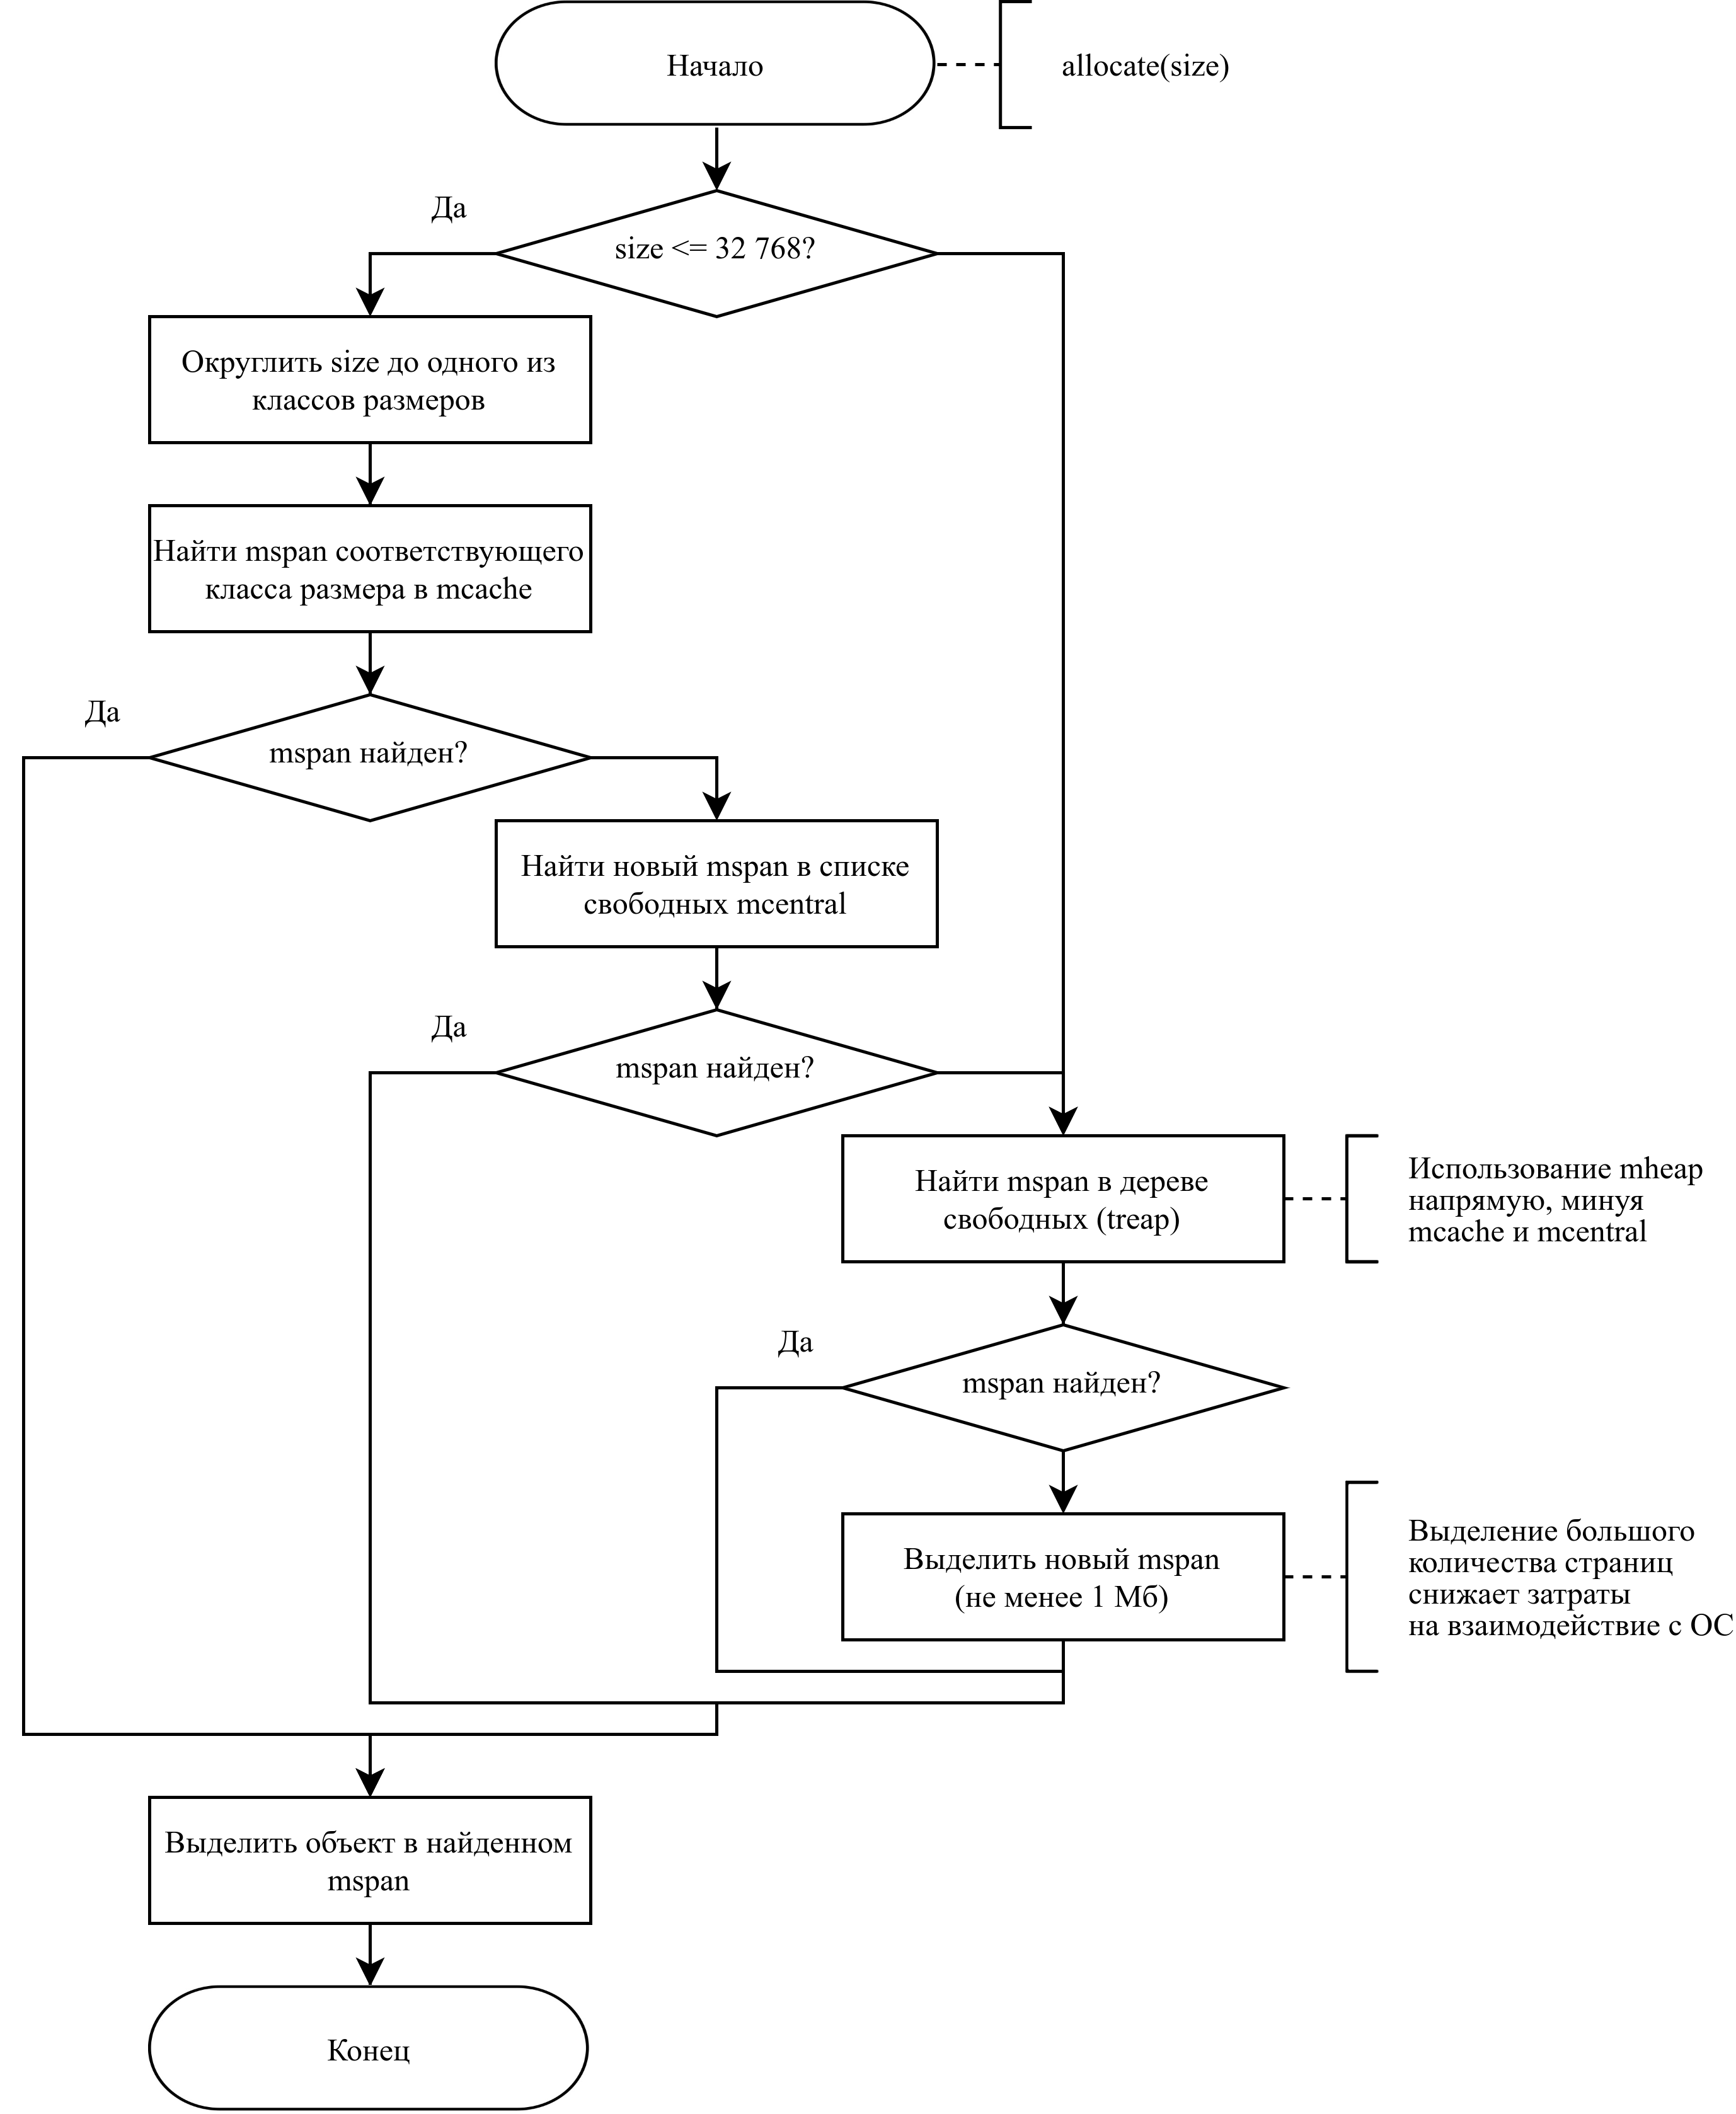
\includegraphics[scale=0.175]{assets/golang-allocate.png}
	\caption{Выделение памяти в куче}
	\label{fig:golang-allocate}
\end{figure}

На рисунке \ref{fig:golang-sweep} показана схема алгоритма освобождения памяти.

\begin{figure}[H]
	\centering
	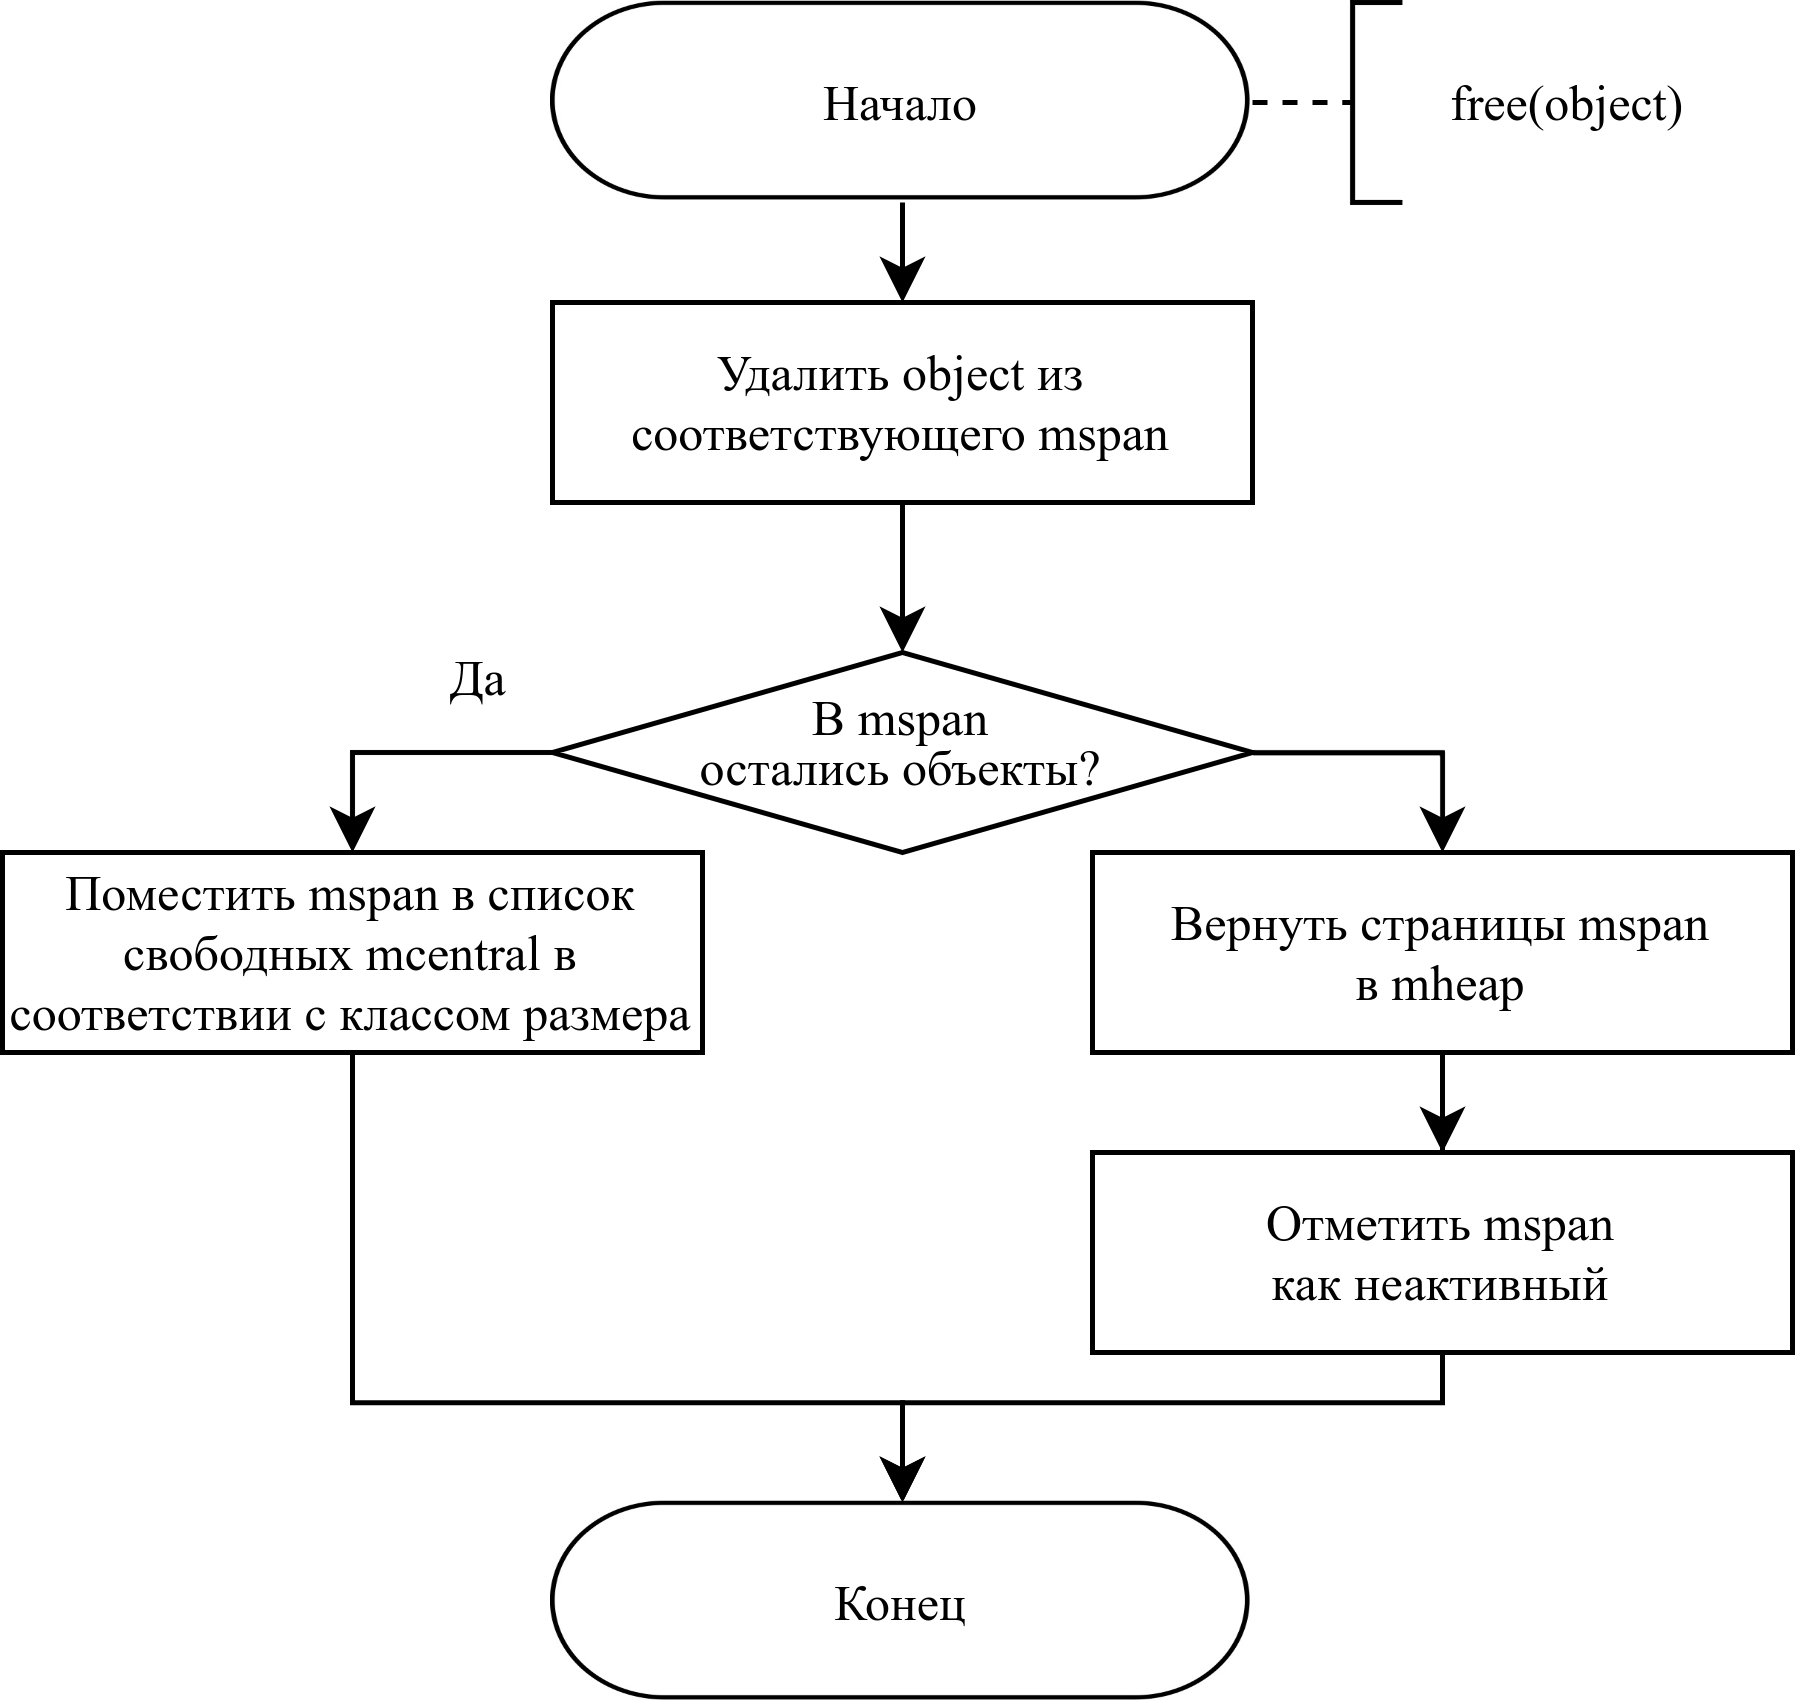
\includegraphics[scale=0.175]{assets/golang-sweep.png}
	\caption{Освобождение памяти в куче}
	\label{fig:golang-sweep}
\end{figure}



\subsection{Структура кучи}

Куча состоит из набора областей, называемых \textbf{аренами} (Arena), размер которых составляет 64 Мб в 64-разрядной версии и 4 Мб в 32-разрядной (heapArenaBytes). Начальный адрес каждой арены также выровнен по размеру арены. \cite{golang_malloc}

С каждой ареной связан объект heapArena \cite{golang_mheap}, который хранит метаданные для этой арены: битовую карту кучи для всех слов (word) в арене и карту span для всех страниц в ней. Объекты heapArena выделяются вне кучи. \cite{golang_malloc}

Структура mheap содержит \textbf{карту арен}, которая охватывает всё доступное адресное пространство программы, поэтому его можно рассматривать как набор арен. Аллокатор старается сохранять арены смежными, чтобы большие span (и, следовательно, большие объекты) могли занимать одновременно несколько арен. \cite{golang_malloc}

Концептуальная схема, отражающая структуру кучи в программе на языке Golang, представлена на рисунке \ref{fig:golang_heap}.

\begin{figure}[H]
	\centering
	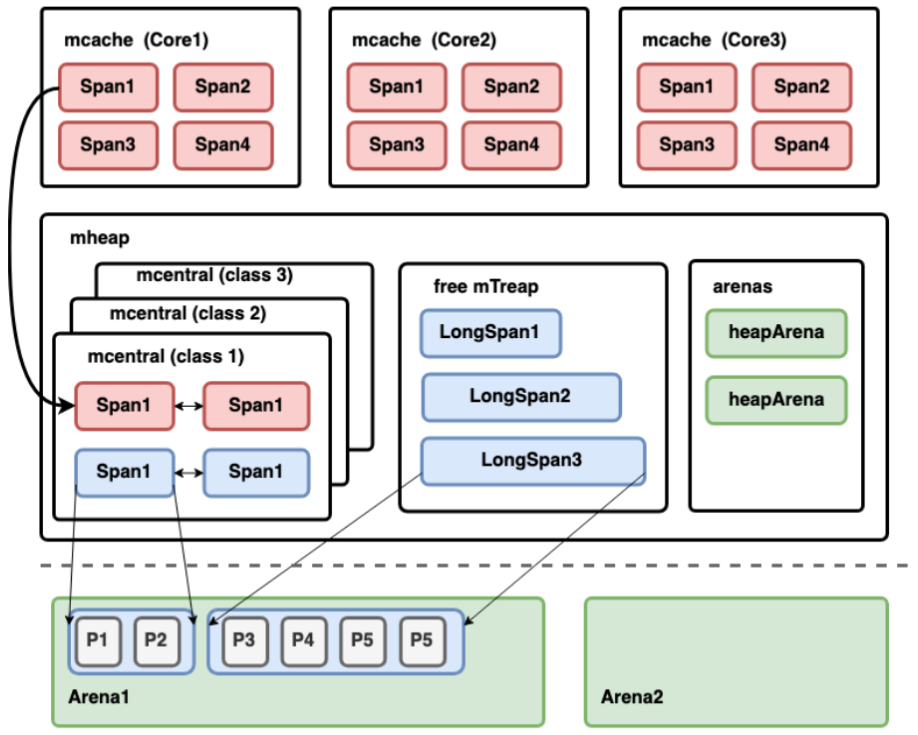
\includegraphics[width=\textwidth]{assets/golang-heap.png}
	\caption{Структура кучи в Golang}
	\label{fig:golang_heap}
\end{figure}



\subsection{Сборка мусора}

В языке Golang для сборки мусора используется алгоритм \textbf{Concurrent Mark-Sweep}, являющийся модификацией алгоритма mark-sweep (см. п. \ref{mark-sweep}), предназначенного для сборки мусора конкурентно с основной программой. \cite{golang_gc}

Сборщик мусора запускается параллельно с потоками основной программы, обладает точностью типов (type accurate, type precise), позволяет нескольким потокам сборки мусора выполняться параллельно. Алгоритм сборки мусора не является уплотняющим и не использует поколения (см. п. \ref{mark-compact} и \ref{generational}). \cite{golang_gc}

Для конкурентной разметки и очистки используются \textbf{барьеры записи} (write barrier), позволяющий избежать ситуации, когда чёрные объекты указывают на белые. Такое может произойти, например, при перемещении указателя в программе до того, как сборщик мусора успел его разметить. В такой ситуации основная программа скрывает объект от сборщика мусора. \cite{golang_gc} Для реализации барьера записи используются операции <<затенения>> (shade), перемещающие указатели программы. Барьер записи затеняет как записываемый указатель, так и записываемое значение при любой записи по указателю \cite{golang_barrier}. 

Ниже представлено описание основных шагов алгоритма сборки мусора.~\cite{golang_gc}

\begin{enumerate}[label*=\arabic*.]
	\item Фаза завершения очистки (sweep termination).
	\begin{enumerate}[label*=\arabic*.]
		\item <<Остановка мира>> (<<stop the world>>, см. п. \ref{mark-sweep}), приводящая к тому, что все потоки достигают \textbf{безопасной точки} (GC safe-point).
		\item Очистка всех мусорных mspan. Неочищенные mspan будут только в том случае, если цикл сборки мусора был запущен раньше ожидаемого времени.
	\end{enumerate}

	\item Фаза разметки (mark).
	\begin{enumerate}[label*=\arabic*.]
		\item Включение барьера записи, постановка в очередь заданий по разметке объектов из корневого набора (см. п. \ref{roots}) и включение ассистентов (assistants), выполняющих свою работу во время выделения памяти. Никакие объекты не могут быть просканированы до тех пор, пока все потоки не включат барьер записи, что достигается с помощью <<остановки мира>>.
		\item <<Запуск мира>> (<<start the world>>). С этого момента работа сборщика мусора выполняется обработчиками разметки (mark workers), запущенными планировщиком, и ассистентами. Выделяемые объекты отмечаются чёрным цветом.
		\item Разметка объектов из корневого набора, включающая в себя сканирование стеков всех горутин, затенение всех глобальных переменных и затенение любых указателей кучи в структурах данных среды выполнения вне кучи. При сканировании стека горутина останавливается, затеняются все указатели, найденные в её стеке, а затем горутина продолжает выполняться.
		\item Очистка рабочей очереди от серых объектов. Каждый серый объект сканируется и отмечается чёрным, затеняя все указатели, найденные в объекте, что, в свою очередь, может привести к добавлению этих указателей в рабочую очередь.
		\item Выполнение алгоритма распределенного завершения (distributed termination algorithm), чтобы определить, когда закончится выполнение заданий разметки объектов из корневого набора или серых объектов.
	\end{enumerate}

	\item Фаза завершения разметки (mark termination).
	\begin{enumerate}[label*=\arabic*.]
		\item <<Остановка мира>>.
		\item Отключение обработчиков и ассистентов.
		\item Очистка, включающая сброс кешей mcache.
	\end{enumerate}

	\item Фаза очистки (sweep).
	\begin{enumerate}[label*=\arabic*.]
		\item Отключение барьера записи.
		\item <<Запуск мира>>. С этого момента выделяемые объекты становятся белыми. Также при необходимости аллокатор может очищать mspan перед использованием.
		\item Выполнение параллельной очистки в фоновом режиме и во время выделения памяти.
	\end{enumerate}
\end{enumerate}

Чтобы предотвратить длительные паузы при сканировании больших объектов и улучшить параллелизм, сборщик мусора разбивает задания сканирования объектов размером более maxObletBytes на \textbf{<<облеты>>}, размер которых не превышает maxObletBytes. Когда при сканировании обнаруживается начало большого объекта, сборщик сканирует только первый фрагмент, а остальные фрагменты помещает в очередь как новые задания сканирования. \cite{golang_gc}



\subsection{Настройка сборщика мусора}

Следующая сборка мусора выполняется после того, как был выделен дополнительный объём памяти, пропорциональный тому который был зафиксирован при предыдущем запуске сборки мусора. Данная пропорция контролируется переменной среды \textbf{GOGC} (по умолчанию  имеет значение 100). Если GOGC=100 и программа использует 4 Мб памяти, следующий цикл сборки мусора запустится тогда, когда объём используемой памяти достигнет 8 Мб. Такая настройка позволяет сохранить линейную зависимость накладных расходов на сборку мусора от накладных расходов на выделение памяти. Настройка GOGC просто изменяет линейную константу. \cite{golang_gc}

По сути GOGC определяет компромисс между накладными расходами памяти и процессорного времени. После каждого цикла сборки мусора определяется целевой размер кучи, а также целевое значение общего размера кучи для запуска следующего цикла. Целевой размер кучи определяется следующим образом. \cite{golang_gc_guide}

\begin{equation}
	Target\ heap = Live\ heap + (Live\ heap + GC\ roots) * GOGC / 100
\end{equation}

Стоит заметить, что данная настройка не учитывает то, что доступная программе память ограничена. В версии Golang 1.19 было добавлено ограничение, которое устанавливает максимальный общий объем памяти (\textbf{GOMEMLIMIT}), который может использовать среда выполнения Golang. \cite{golang_1_19} \cite{golang_proposal_limit}

Поскольку сборщик мусора имеет явный контроль над тем, сколько памяти кучи используется программой, он устанавливает общий размер кучи на основе этого ограничения памяти и того, сколько другой памяти использует среда выполнения Golang. Когда размер используемой памяти достигает пикового значения, определенного GOGC, сборщик мусора запускается чаще, чтобы поддерживать его в пределах лимита. \cite{golang_gc_guide}

Стоить заметить, что даже когда GOGC отключен, ограничение памяти всё равно соблюдается. Это позволяет достичь максимальной экономии ресурсов, поскольку устанавливается мини \cite{golang_gc_guide}мальная частота запуска сборщика мусора, необходимая для поддержания ограничения памяти.

Несмотря на то, что ограничение памяти, очевидно, является мощным инструментом, его использование не обходится без накладных расходов и, конечно же, не отменяет полезность GOGC. \cite{golang_gc_guide}

Такая ситуация, когда программа не может выполняться из-за постоянных циклов сборки мусора, называется \textbf{перегрузкой}. Во многих случаях неопределённая остановка хуже, чем нехватка памяти, которая обычно приводит к гораздо более быстрому сбою. По этой причине ограничение памяти в Golang определяется как \textbf{мягкое} (soft memory limit) \cite{golang_proposal_limit}. Среда выполнения Go не дает никаких гарантий, что она сохранит заданный лимит памяти при любых обстоятельствах, а только обещает некоторое разумное количество усилий. Это ослабление ограничения памяти имеет решающее значение для предотвращения зависаний, поскольку оно позволяет аллокатору превысить предел, чтобы не тратить слишком много времени на сборку мусора. \cite{golang_gc_guide}

В языке Golang мягкое ограничение памяти реализовано следующим образом: сборщик мусора устанавливает верхний предел количества процессорного времени, которое он может использовать в течение некоторого временного промежутка (окна, frame). В настоящее время этот предел установлен примерно на уровне 50\%. В случае неправильной настройки лимита памяти, когда по ошибке он был установлен слишком низким, программа замедлится максимум в 2 раза, поскольку GC не может отнять у неё более 50\% процессорного времени. \cite{golang_gc_guide}


\subsection{Арены памяти}

В версии Golang 1.20 появилось экспериментальное решение для управления памятью, которое позволяет совместить безопасное выделение динамической памяти и уменьшение влияния среды выполнения языка, включающей интегрированный менеджер памяти, на производительность приложения.

% С точки зрения распределения памяти работа с ареной похожа на выделение одной области памяти (который может увеличиваться в размере) и при освобождении арены все выделенные в ней объекты становятся недоступными.

Пакет arena предоставляет возможность выделения памяти в программах на языке Golang и освобождать её вручную, причем безопасно и одновременно. Цель этой функциональности --- повышение эффективности программ: освобождение памяти вручную откладывает следующий цикл сборки мусора. В свою очередь, снижение частоты циклов означает уменьшение накладных расходов на сборку мусора. \cite{golang_arena_cource}

Большая часть описанной функциональности рассматриваемого пакета реализована в типе Arena, который является абстракцией относительно большого объёма памяти, выделенного в куче. Наиболее эффективное использование Arena достигается при хранении в них некоторого множества объектов программы, занимающих около 1 Мб памяти. \cite{golang_arena_cource} \cite{golang_arena_proposal}

Стоит заметить, что при использовании этой ограниченной формы ручного выделения памяти возможны ошибки типа <<use-after-free>> (использование после освобождения). Пакет Arena ограничивает влияние этих ошибок, предотвращая повторное использование освобождённых областей памяти до тех пор, пока сборщик мусора не сможет убедиться в том, что это безопасно. Как правило, ошибка <<use-after-free>> приводит к сбою и получению сообщения об ошибке, но пакет Arena оставляет за собой право не вызывать сбой программы при использовании освобождённой памяти. Это означает, что реализация данного пакета допускает выделение памяти так, как это обычно делает среда выполнения, оставляя за собой право иногда делать это для некоторых объектов программы.~\cite{golang_arena_cource}

Повышение производительности программы, использующей выделение памяти на аренах, можно ожидать в тех случаях, когда приложение интенсивно выделяет память (например, при работе с ссылочными структурами данных, такими как двоичные деревья), но при этом предполагается, что выделенные структуры данных являются относительно долгоживущими и существуют до момента освобождения арены целиком (сборщик мусора для арены не применяется и выделенные на ней объекты не освобождаются автоматически). 


%Мои конспекты в Obsidian
%
%Лекция
%
%https://habr.com/ru/companies/oleg-bunin/articles/676332/
%
%https://go101.org/article/memory-block.html
%
%https://go.dev/ref/mem
%
%https://go.dev/doc/gc-guide
%
%https://github.com/golang/proposal/blob/master/design/48409-soft-memory-limit.md (ALSO FOR JAVA)
%
%https://github.com/golang/go/issues/51317
%
%https://backendinterview.ru/goLang/memory.html
%
%
%
%https://medium.com/safetycultureengineering/an-overview-of-memory-management-in-go-9a72ec7c76a8
%https://medium.com/@ali.can/memory-optimization-in-go-23a56544ccc0
